\documentclass{article}
\usepackage{ctex}

\title{数字逻辑与计算机组成\\ {\small 实验 1: 基本逻辑部件设计}}
\author{王卫东\quad 221900332}
\date{\zhtoday}

\usepackage{hyperref}
\usepackage{algorithm}
\usepackage{algorithmicx}
\usepackage{algpseudocode}
\usepackage{float}  
\usepackage{lipsum}
\usepackage{color, xcolor}
\usepackage{listings}
\usepackage{dirtree}
\usepackage{ulem}
\usepackage{graphicx}
\usepackage{amsmath}
\usepackage{amssymb}
\usepackage{amsfonts}
\usepackage{xcolor}
\usepackage{tikz}
\usepackage{zhnumber} % change section number to chinese
\renewcommand\thesection{\zhnum{section}}
\renewcommand\thesubsection{\arabic{subsection}}
\usetikzlibrary{arrows,shapes,chains}

\begin{document}
    \maketitle

    \section{实验目的}

    \begin{enumerate}
        \item 熟悉 Logisim 软件的使用方法。
        \item 掌握使用晶体管实现基本逻辑部件的方法。
        \item 利用基础元器件库设计简单数字电路。
        \item 掌握子电路的设计和应用。
        \item 掌握分线器、隧道、探针等 Logisim 组件的使用方法。
    \end{enumerate}

    \section{实验环境}

    Logisim:https://github.com/Logisim-Ita/Logisim

    \section{实验内容}
    
    \subsection{利用基本逻辑门设计一个3输入多数表决器}

    \subsubsection{整体方案设计}
    \begin{figure}[H]
    \centering
    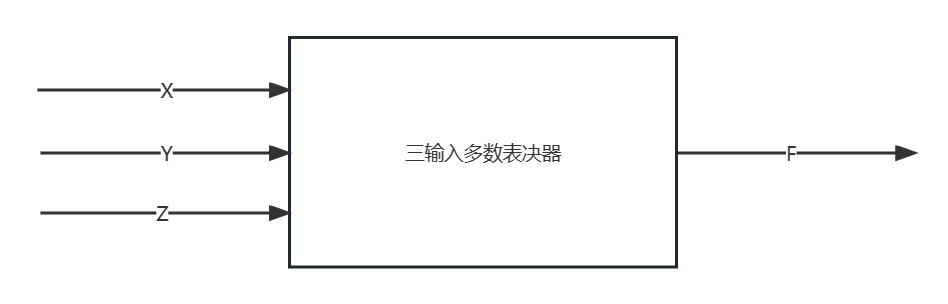
\includegraphics[width=0.8\textwidth]{1.1.jpg}
    \caption{3输入多数表决器整体方案设计}
    \end{figure}

    \subsubsection{顶层模块设计}
    实验电路较简单,不需要顶层模块设计图。

    \subsubsection{输入输出引脚}
    \begin{table}[H]
    \centering
    \begin{tabular}{|c|c|}
        \hline
        XYZ & 输入引脚 \\ \hline
        F   & 输出引脚 \\ \hline
    \end{tabular}
    \caption{3输入多数表决器引脚作用}
    \end{table}

    \subsubsection{原理图和电路图}
    \begin{figure}[H]
    \centering
    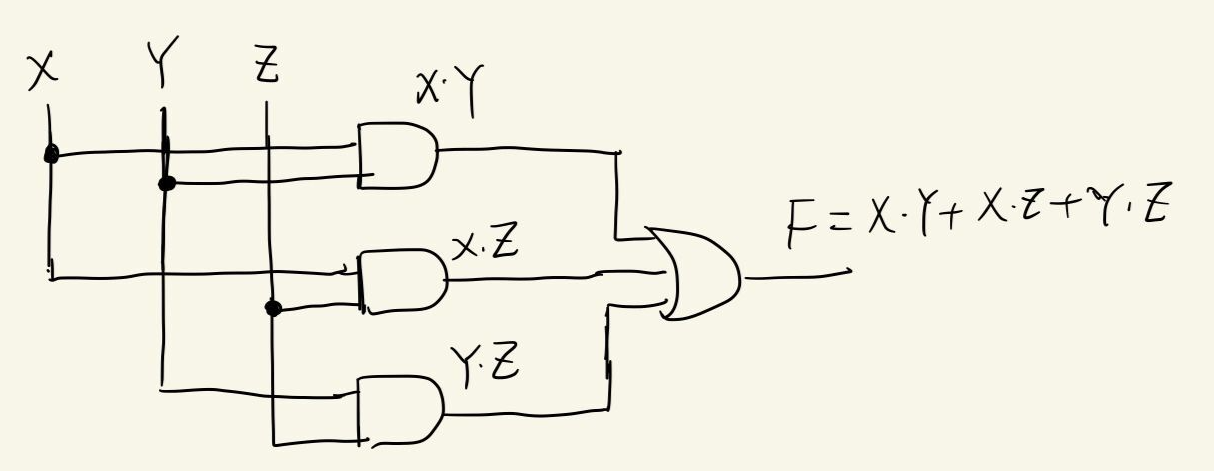
\includegraphics[width=0.8\textwidth]{1.3.png}
    \caption{3输入多数表决器原理图}
    \end{figure}

    \begin{figure}[H]
    \centering
    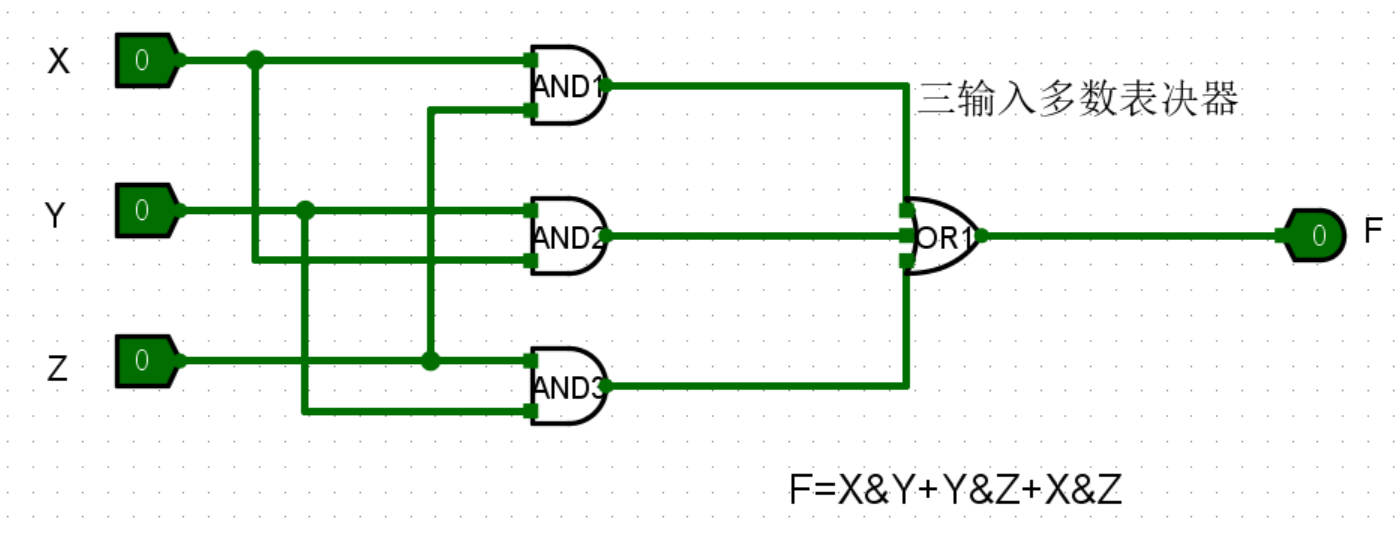
\includegraphics[width=0.8\textwidth]{1.2.png}
    \caption{3输入多数表决器电路图}
    \end{figure}

    \subsubsection{仿真测试图}
    \begin{figure}[H]
    \centering
    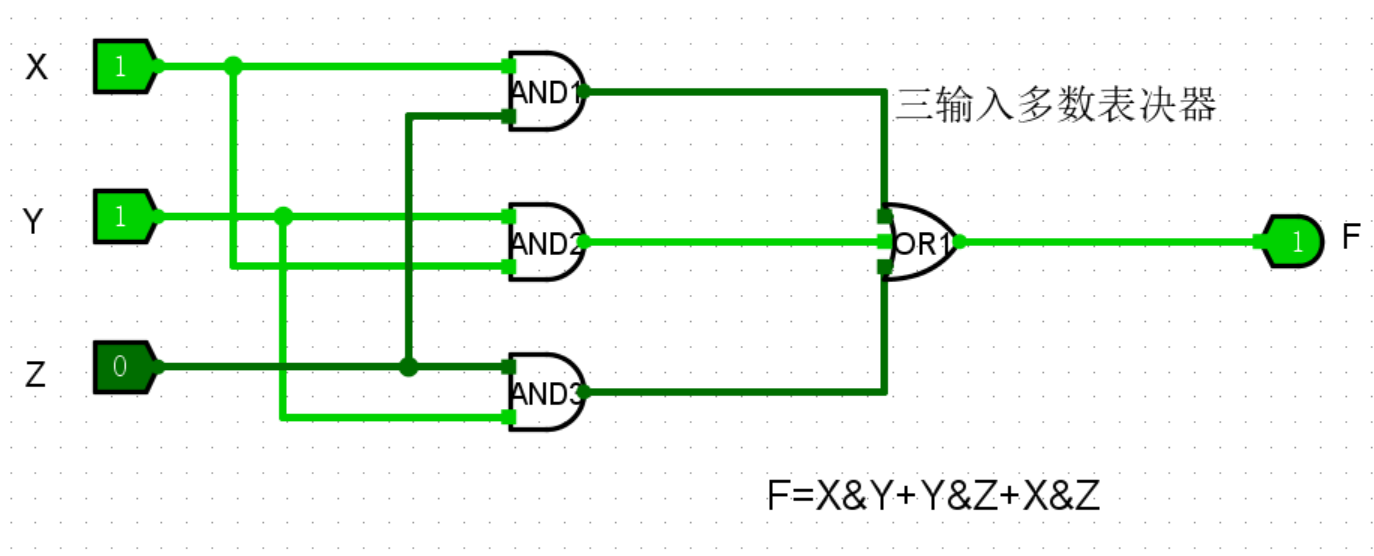
\includegraphics[width=0.4\textwidth]{1.4.1.png}
    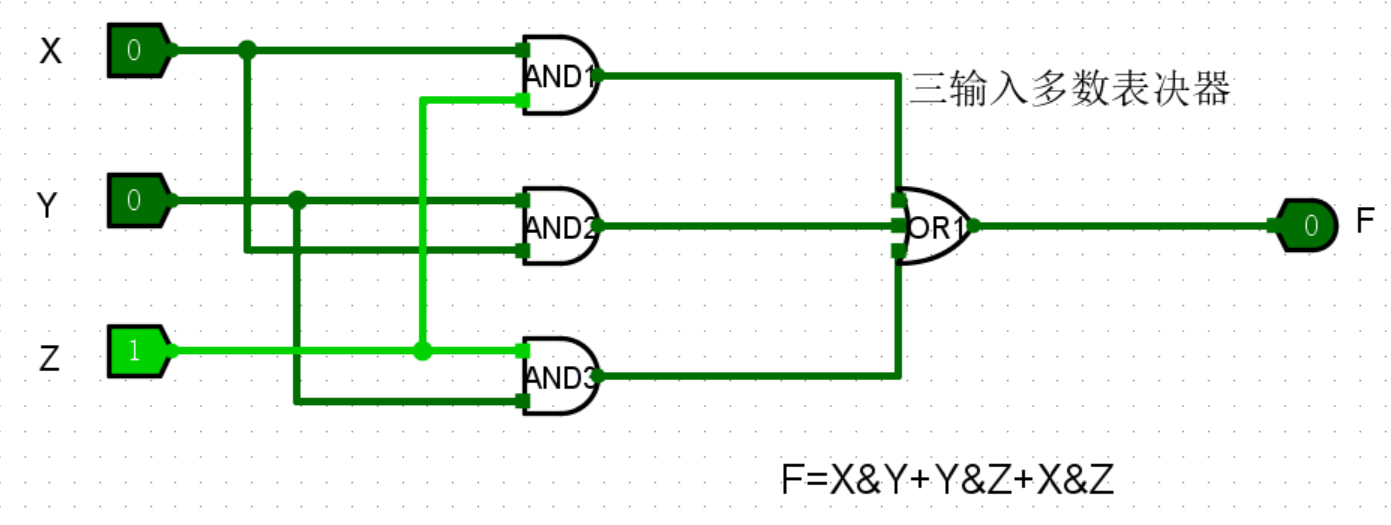
\includegraphics[width=0.4\textwidth]{1.4.2.png}
    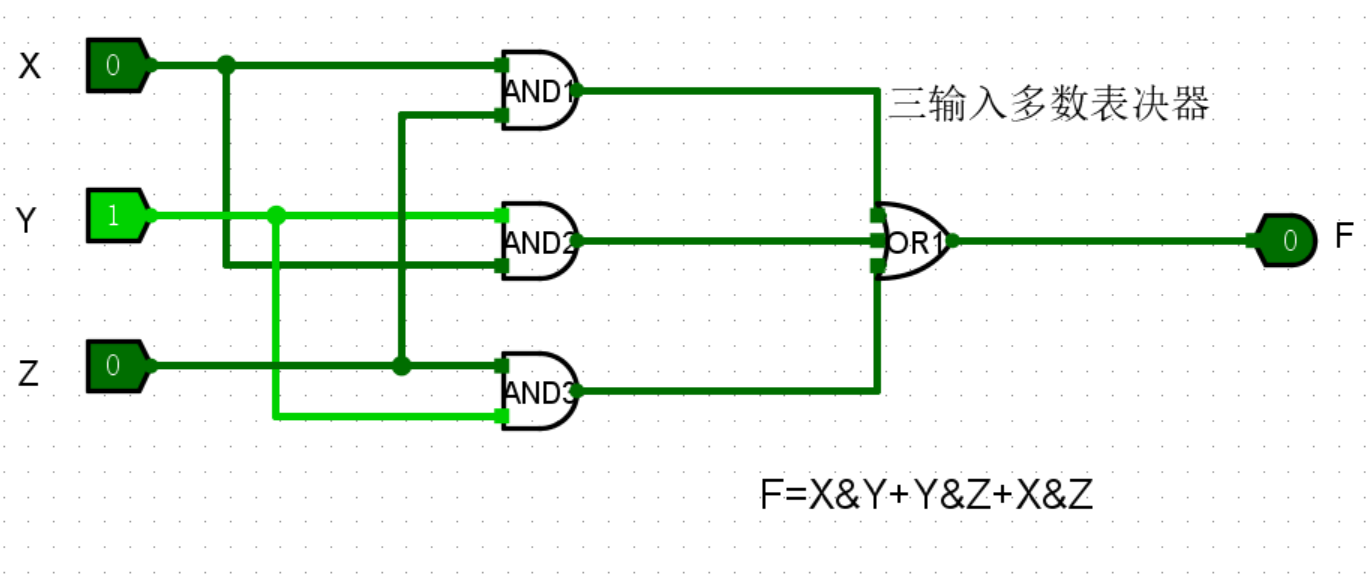
\includegraphics[width=0.4\textwidth]{1.4.3.png}
    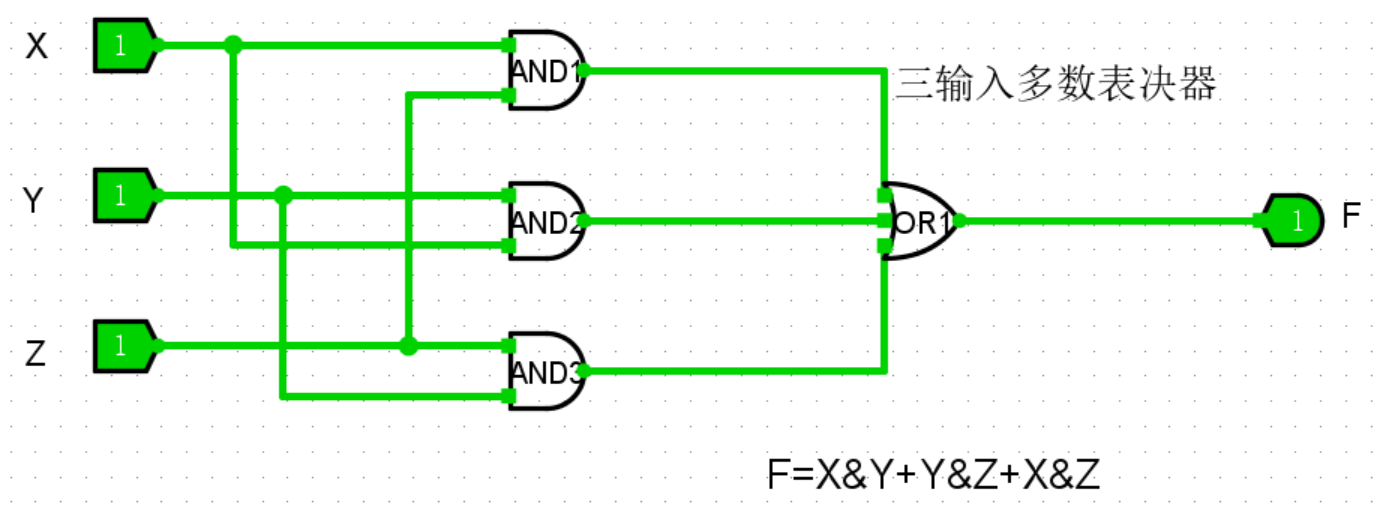
\includegraphics[width=0.4\textwidth]{1.4.4.png}
    \caption{3输入多数表决器仿真测试图}
    \end{figure}

    \begin{table}[H]
    \centering
    \begin{tabular}{|c c c|c|}
        \hline
        X & Y & Z & F \\ \hline
        0 & 0 & 0 & 0 \\ \hline
        0 & 0 & 1 & 0 \\ \hline
        0 & 1 & 0 & 0 \\ \hline
        0 & 1 & 1 & 1 \\ \hline
        1 & 0 & 0 & 0 \\ \hline
        1 & 0 & 1 & 1 \\ \hline
        1 & 1 & 0 & 1 \\ \hline
        1 & 1 & 1 & 1 \\ \hline
    \end{tabular}
    \caption{3输入多数表决器真值表}
    \end{table}

    \subsubsection{错误现象及分析}
    在完成实验的过程中,没有遇到任何错误。
    
    \subsection{利用CMOS晶体管构建两输入或门,并验证其功能}

    \subsubsection{整体方案设计}
    \begin{figure}[H]
    \centering
    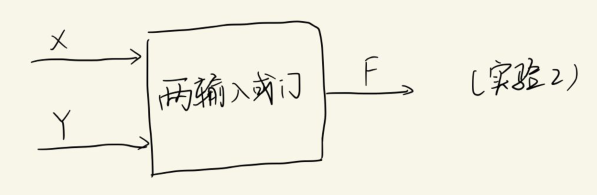
\includegraphics[width=0.8\textwidth]{2.1.png}
    \caption{2输入或门整体方案设计}
    \end{figure}
    
    \subsubsection{顶层模块设计}
    实验电路较为简单,不需要顶层模块设计图。

    \subsubsection{输入输出引脚}
    \begin{table}[H]
    \centering
    \begin{tabular}{|c|c|}
        \hline
        XY & 输入引脚 \\ \hline
        F   & 输出引脚 \\ \hline
    \end{tabular}
    \caption{2输入或门引脚作用}
    \end{table}

    \subsubsection{原理图和电路图}
    \begin{figure}[H]
    \centering
    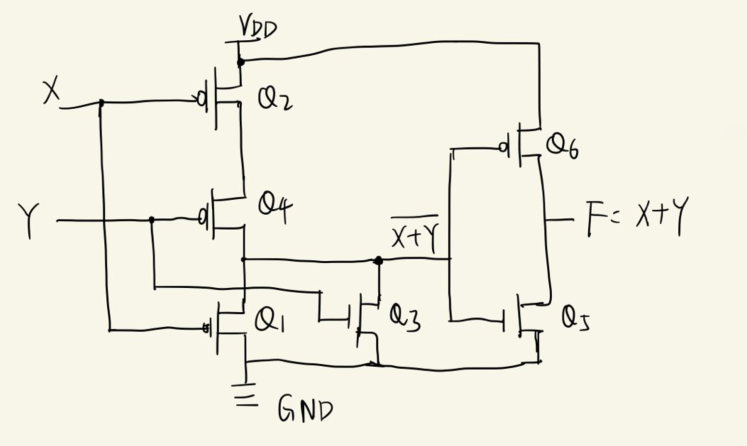
\includegraphics[width=0.8\textwidth]{2.4.png}
    \caption{2输入或门原理图}
    \end{figure}

    \begin{figure}[H]
    \centering
    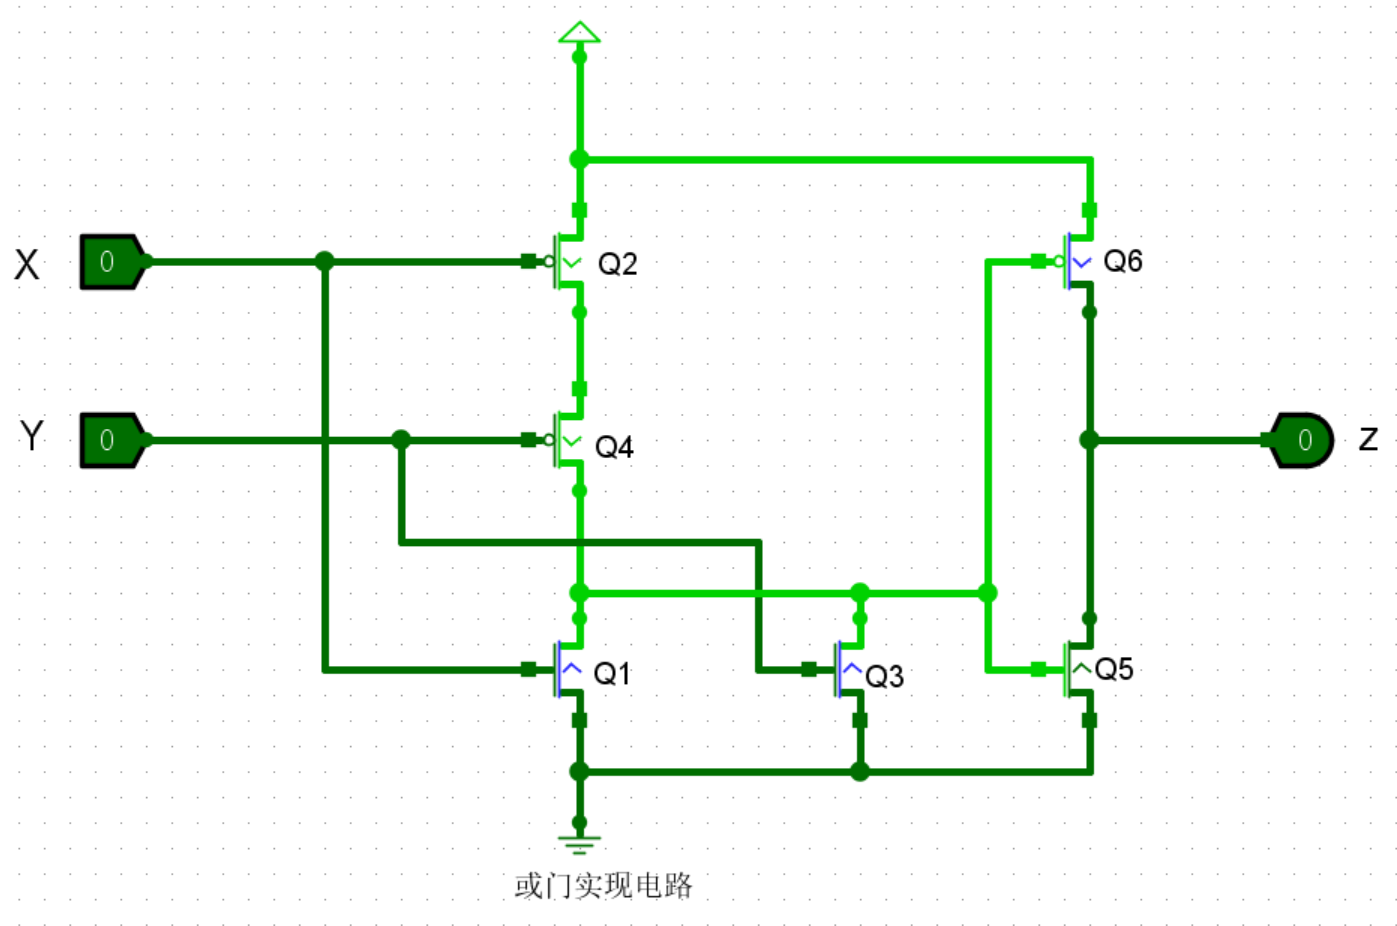
\includegraphics[width=0.8\textwidth]{2.4.2.png}
    \caption{2输入或门电路图}
    \end{figure}

    \subsubsection{仿真测试图}
    \begin{figure}[H]
    \centering
    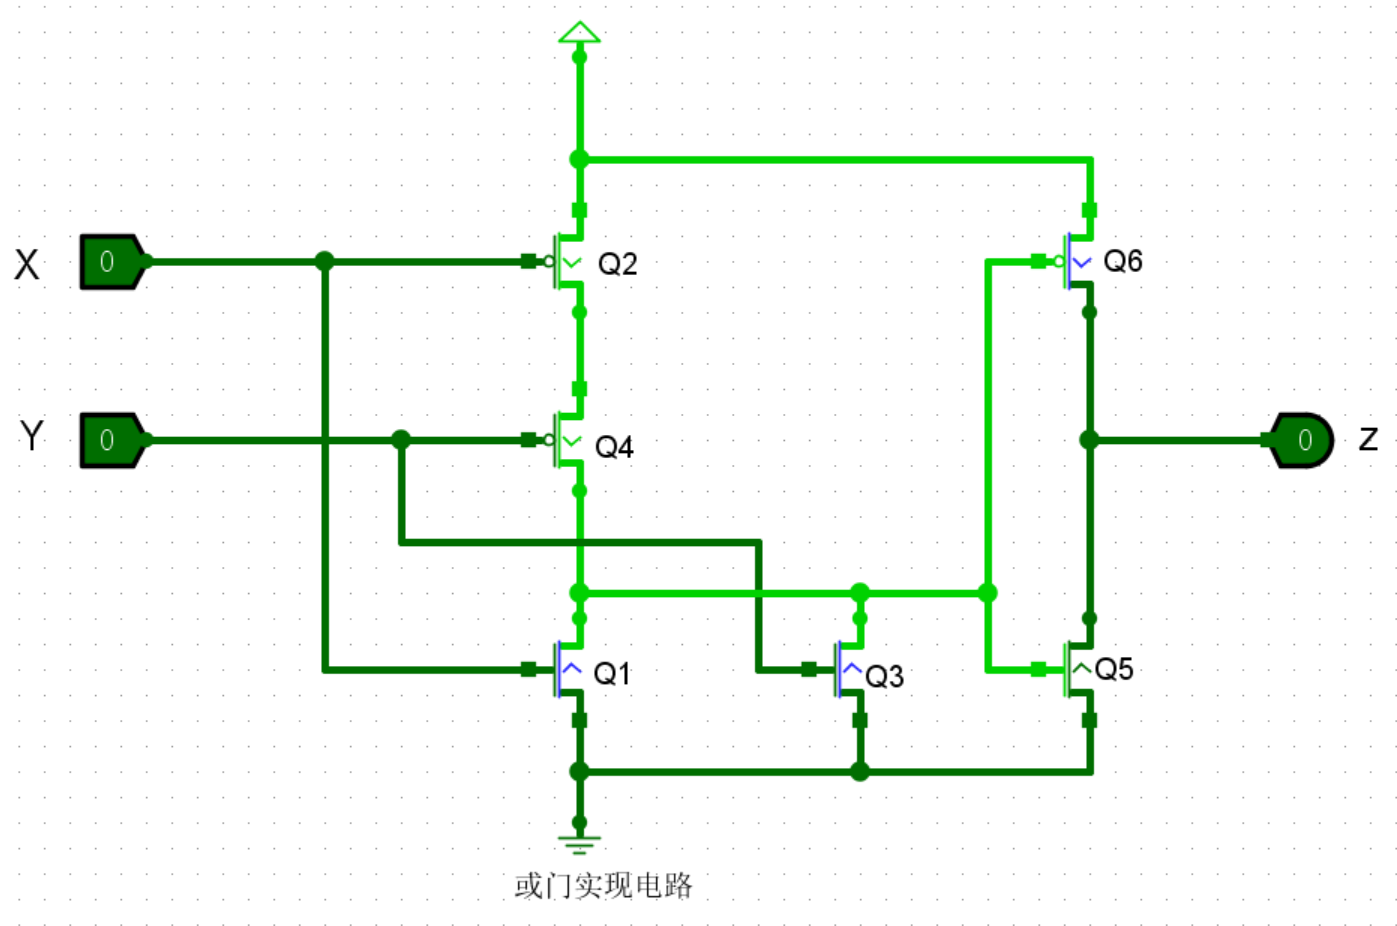
\includegraphics[width=0.4\textwidth]{2.5.1.png}
    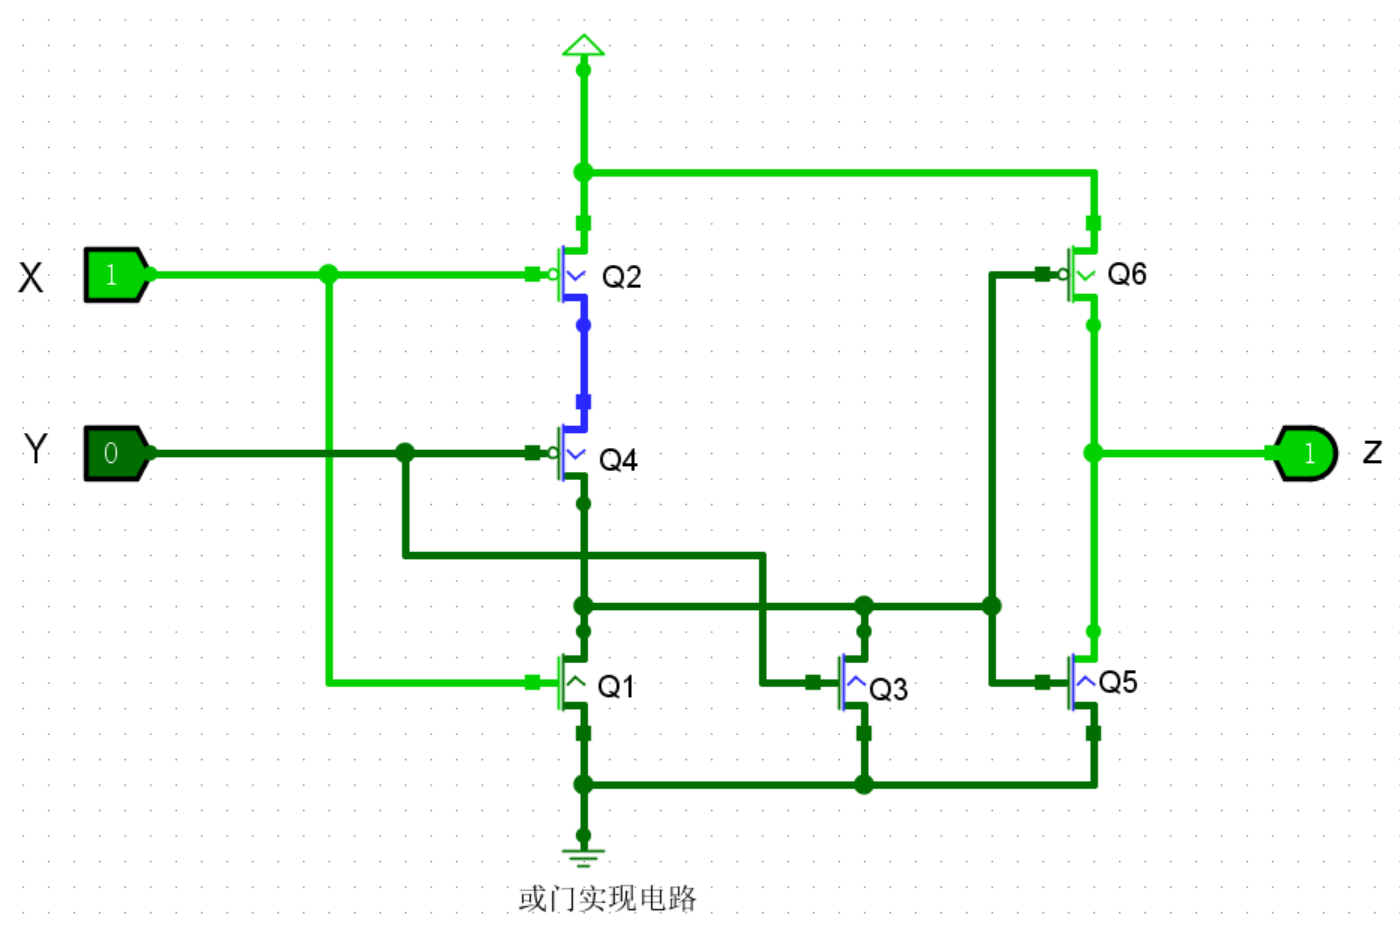
\includegraphics[width=0.4\textwidth]{2.5.2.png}
    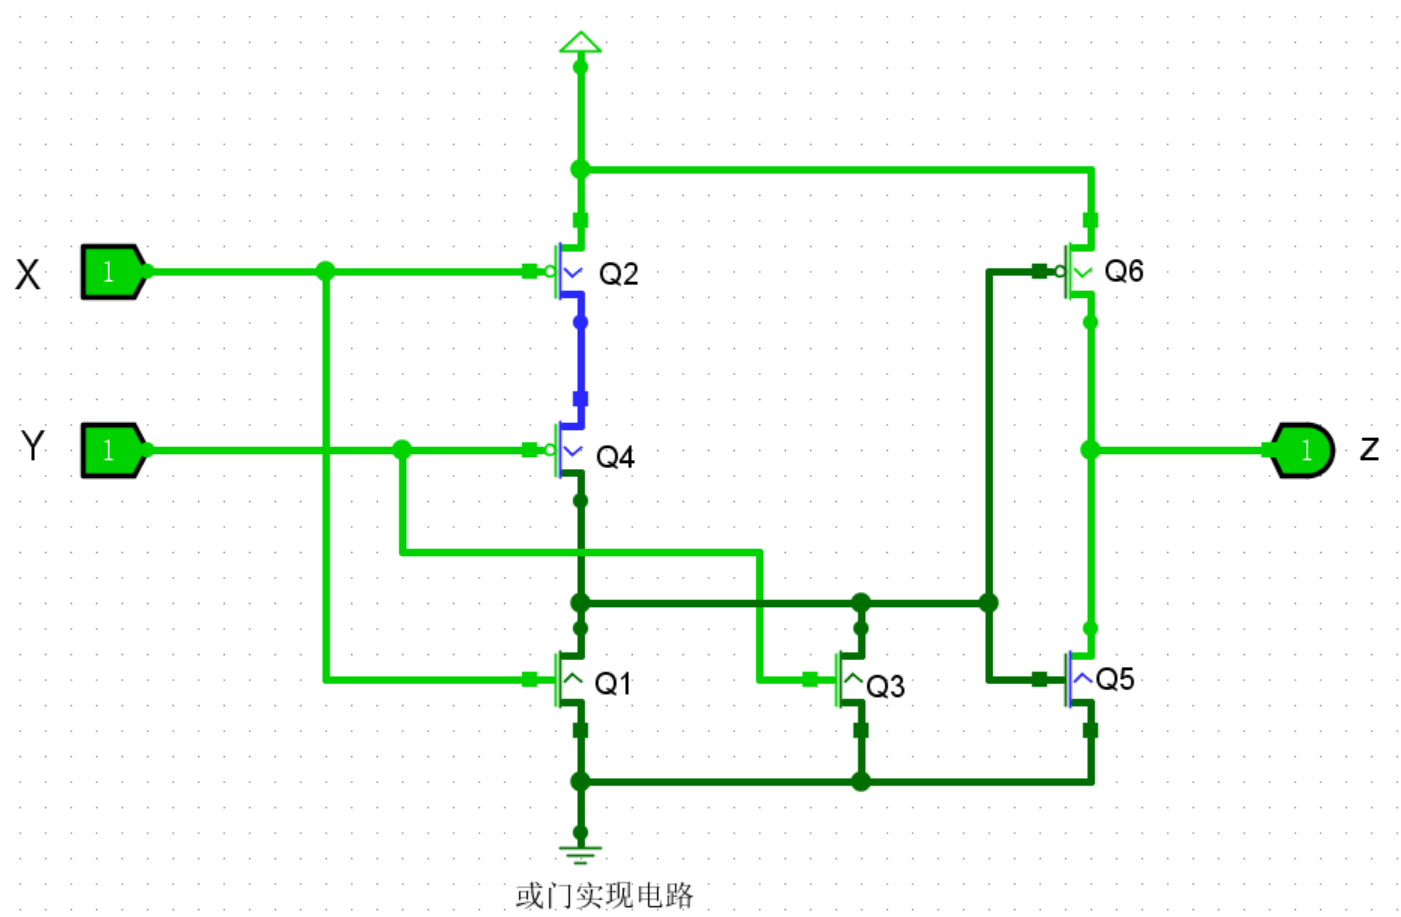
\includegraphics[width=0.4\textwidth]{2.5.3.png}
    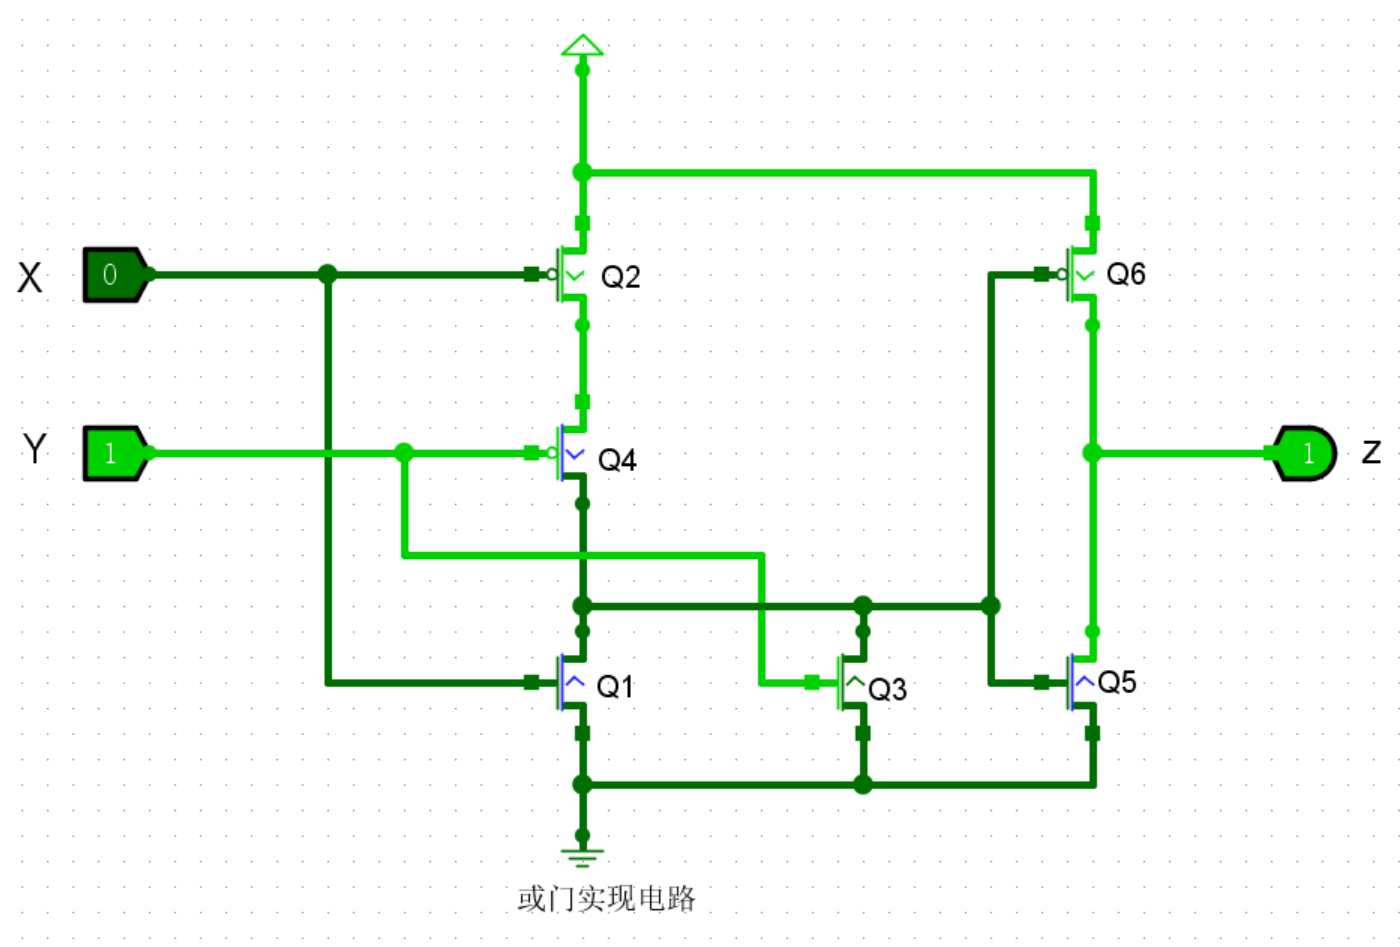
\includegraphics[width=0.4\textwidth]{2.5.4.png}
    \caption{2输入或门仿真测试}
    \end{figure}

    \begin{table}[H]
    \centering
    \begin{tabular}{|c c|c|}
        \hline
        X & Y & F \\ \hline
        0 & 0 & 0 \\ \hline
        0 & 1 & 1 \\ \hline
        1 & 0 & 1 \\ \hline
        1 & 1 & 1 \\ \hline
    \end{tabular}
    \caption{2输入或门真值表}
    \end{table}

    \subsubsection{错误现象及分析}
    在完成实验的过程中,有地方出现红线,经检查是因为P-MOS管用成了N-MOS管。

    \subsection{利用基本逻辑门和CMOS晶体管实现多路选择器,并进行静态冒险检测}

    \subsubsection{整体方案设计}
    \begin{figure}[H]
    \centering
    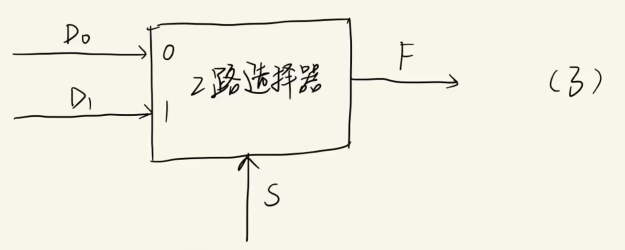
\includegraphics[width=0.8\textwidth]{3.1.png}
    \caption{多路选择器整体方案设计}
    \end{figure}
    
    \subsubsection{顶层模块设计}
    实验电路较为简单,不需要顶层模块设计图。

    \subsubsection{输入输出引脚}
    \begin{table}[H]
    \centering
    \begin{tabular}{|c|c|}
        \hline
        D0 D1 & 输入引脚 \\ \hline
        S & 使能端 \\ \hline 
        F   & 输出引脚 \\ \hline
    \end{tabular}
    \caption{多路选择器引脚作用}
    \end{table}

    \subsubsection{原理图和电路图}
    \begin{figure}[H]
    \centering
    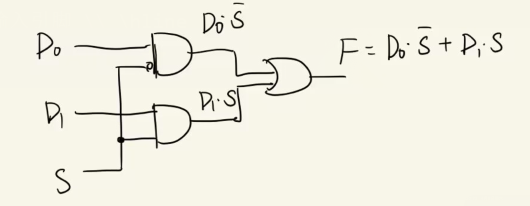
\includegraphics[width=0.8\textwidth]{3.4.1.png}
    \caption{多路选择器原理图}
    \end{figure}

    \begin{figure}[H]
    \centering
    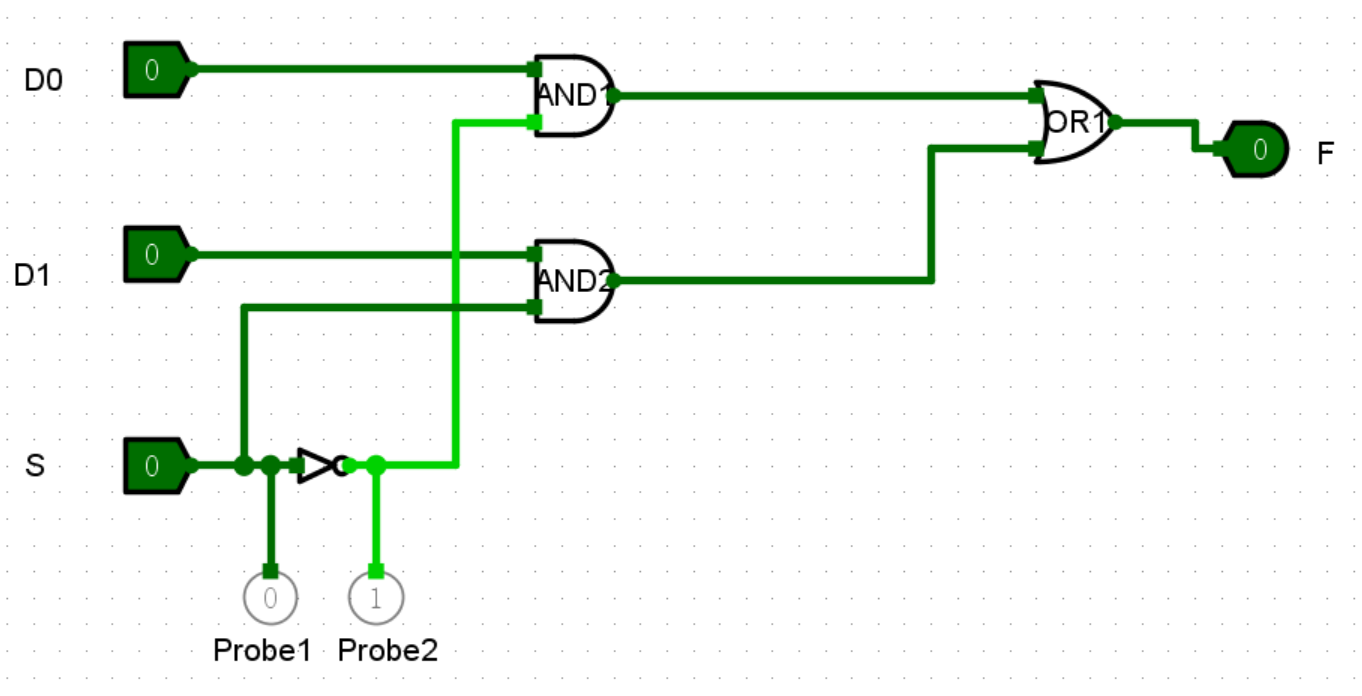
\includegraphics[width=0.8\textwidth]{3.4.2.png}
    \caption{多路选择器电路图}
    \end{figure}

    \subsubsection{仿真测试图}
    \begin{figure}[H]
    \centering
    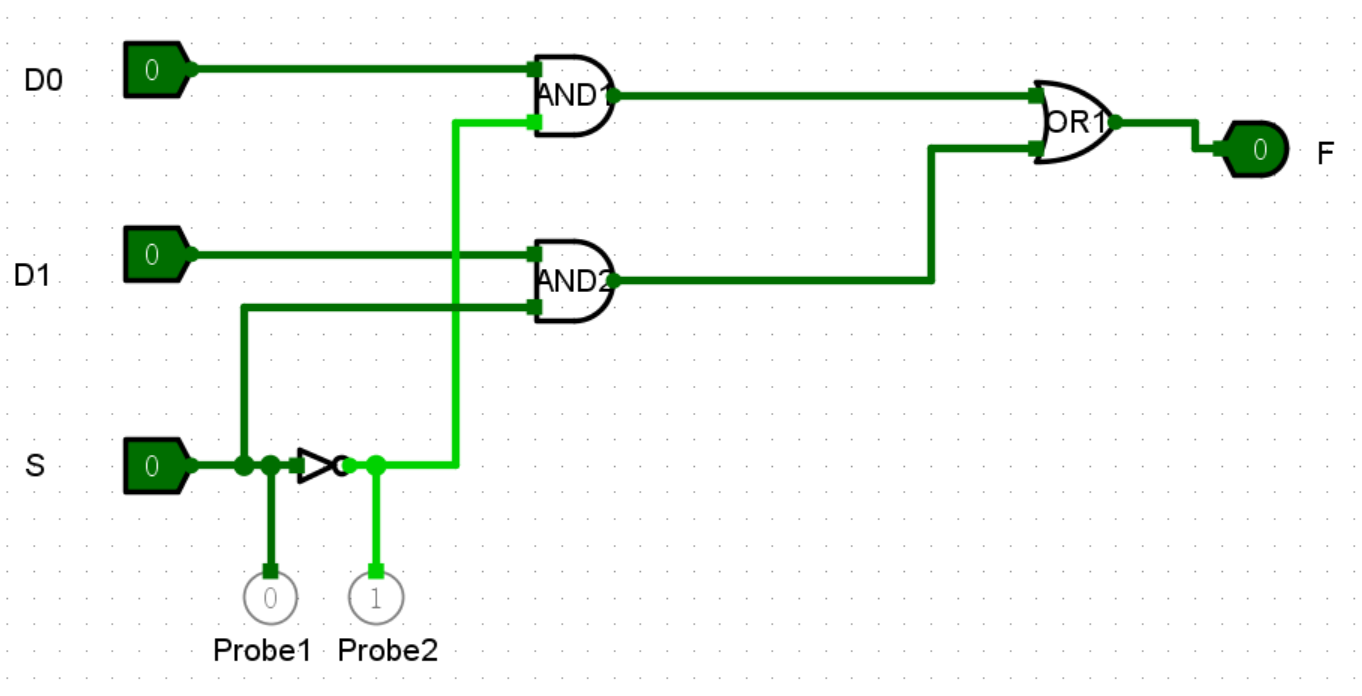
\includegraphics[width=0.4\textwidth]{3.5.1.png}
    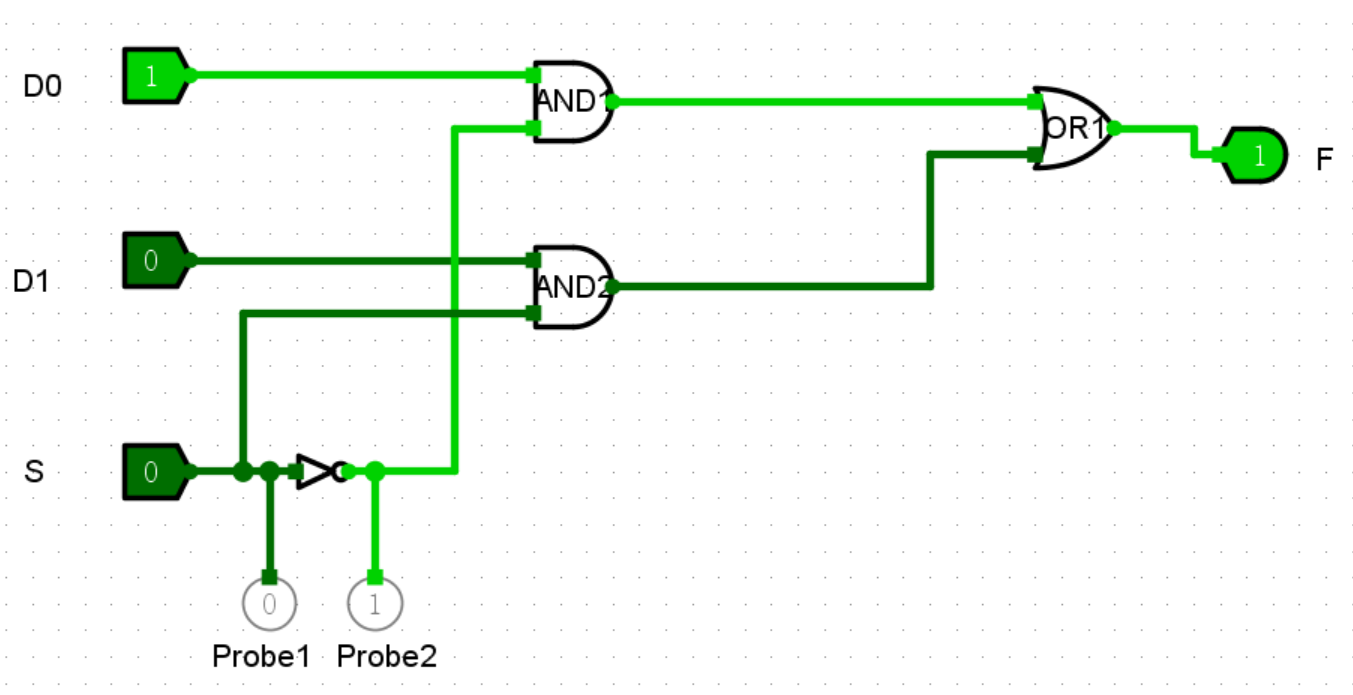
\includegraphics[width=0.4\textwidth]{3.5.2.png}
    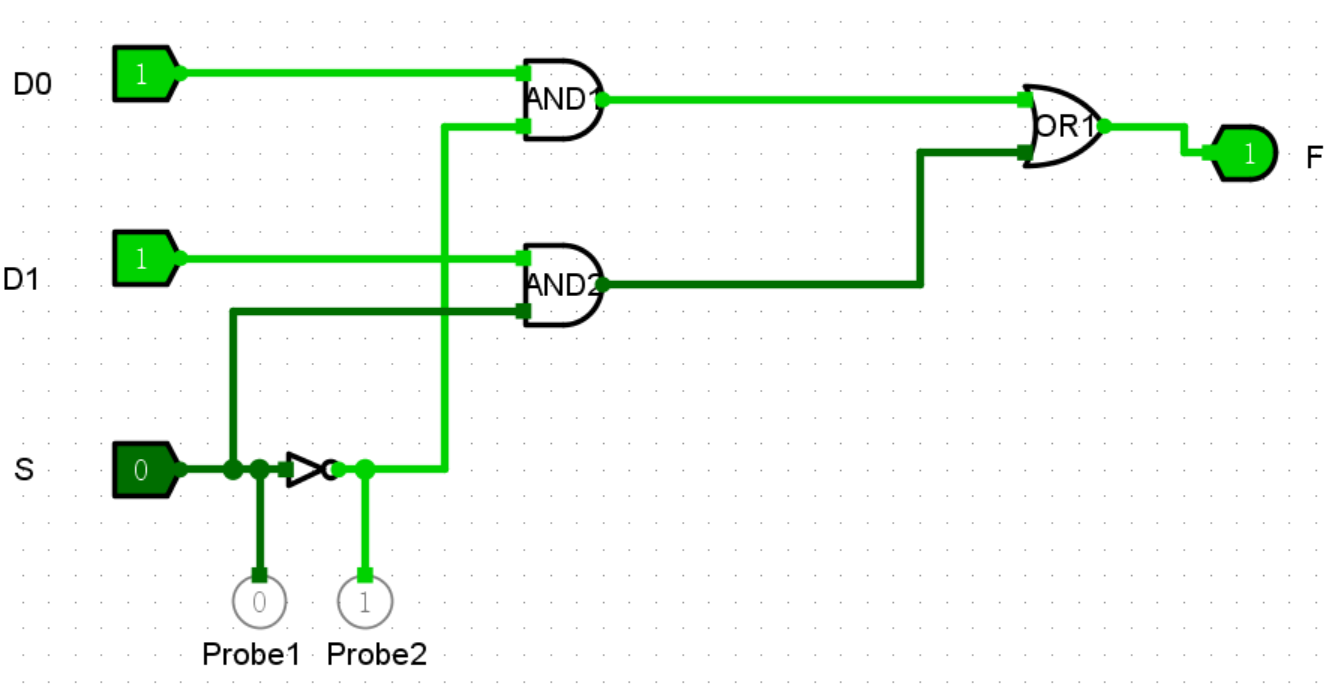
\includegraphics[width=0.4\textwidth]{3.5.3.png}
    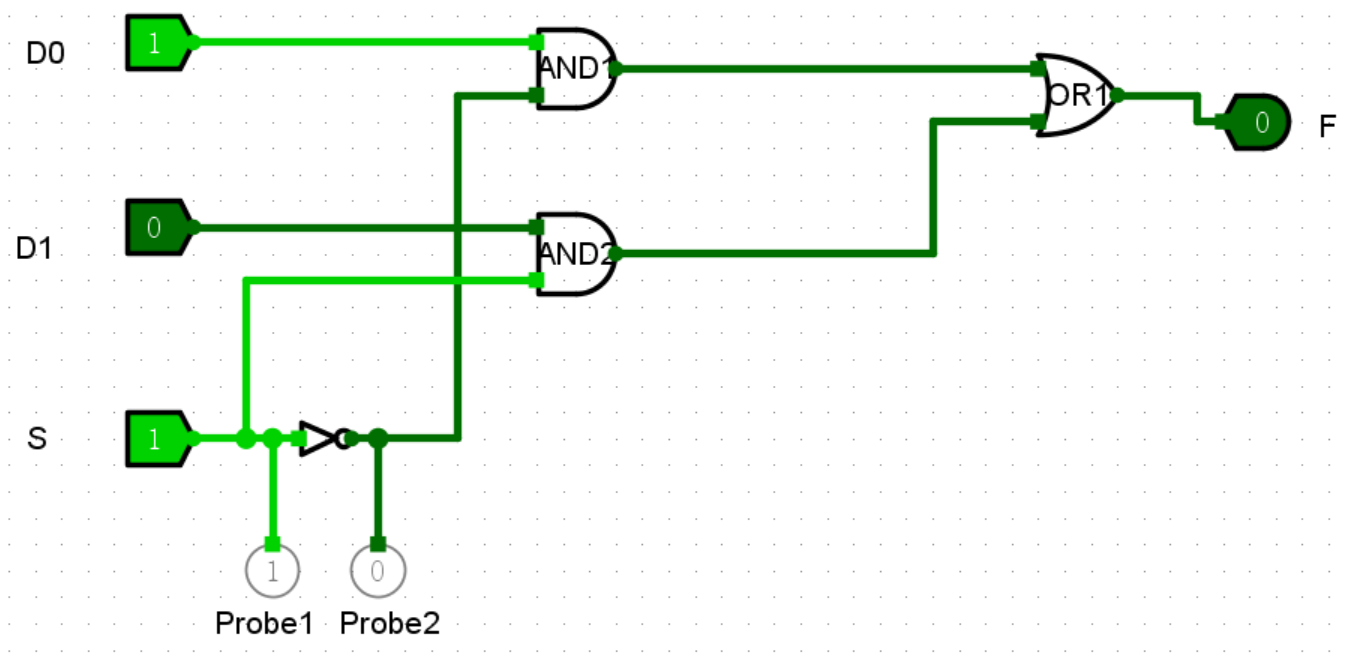
\includegraphics[width=0.4\textwidth]{3.5.4.png}
    \caption{多路选择器仿真测试图}
    \end{figure}

    \begin{table}[H]
    \centering
    \begin{tabular}{|c c c|c|}
        \hline
        D0 & D1 & S & F \\ \hline
        0 & 0 & 0 & 0 \\ \hline
        0 & 0 & 1 & 0 \\ \hline
        0 & 1 & 0 & 0 \\ \hline
        0 & 1 & 1 & 1 \\ \hline
        1 & 0 & 0 & 1 \\ \hline
        1 & 0 & 1 & 0 \\ \hline
        1 & 1 & 0 & 1 \\ \hline
        1 & 1 & 1 & 1 \\ \hline
    \end{tabular}
    \caption{3输入多路选择器真值表}
    \end{table}

    \subsubsection{静态冒险检测}
    下面进行静态冒险检测。当 $D0$ 和 $D1$ 都是 1 时,逻辑表达式为 $F = S + \bar{S} $。此时,当
    $S$ 由 1 变为 0 时,由于 $S → \bar{S}  → AND1 → OR1 $的传输延迟比 $S → AND2 → OR1$ 的传输
    延迟要大,所以会出现 $F$ 由 1 短暂变为 0 再变为 1 的静态冒险。关闭 Simulate - Simulate
    Enable, 进行若干次 Simulate - Step Simulate,测试图如下图所示。
    \begin{figure}[H]
        \centering
        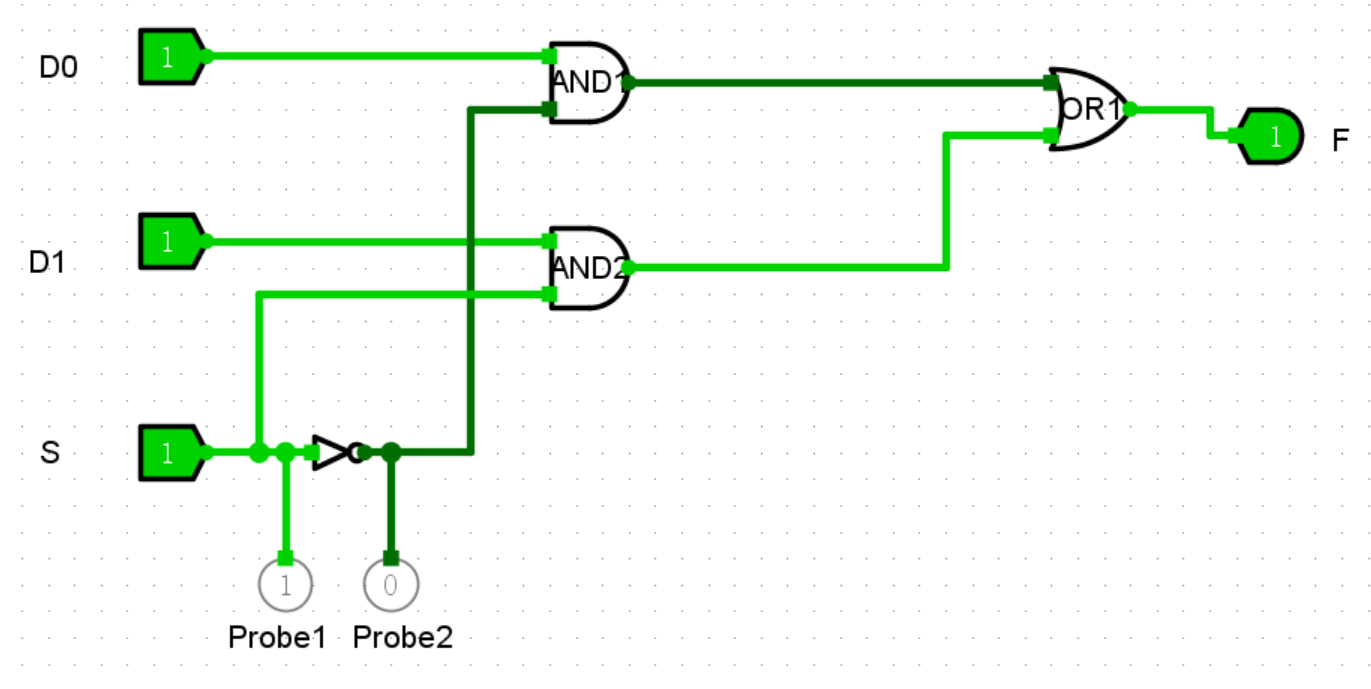
\includegraphics[width=0.4\textwidth]{3.6.1.png}
        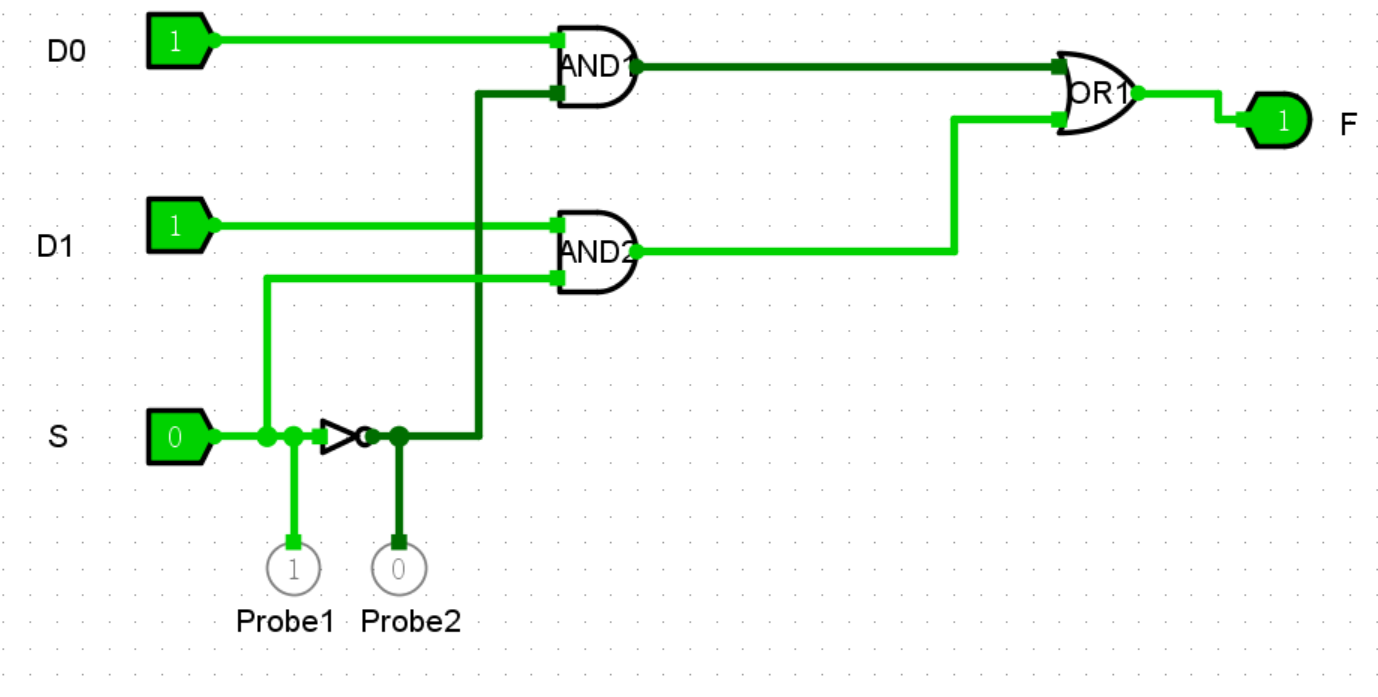
\includegraphics[width=0.4\textwidth]{3.6.2.png}
        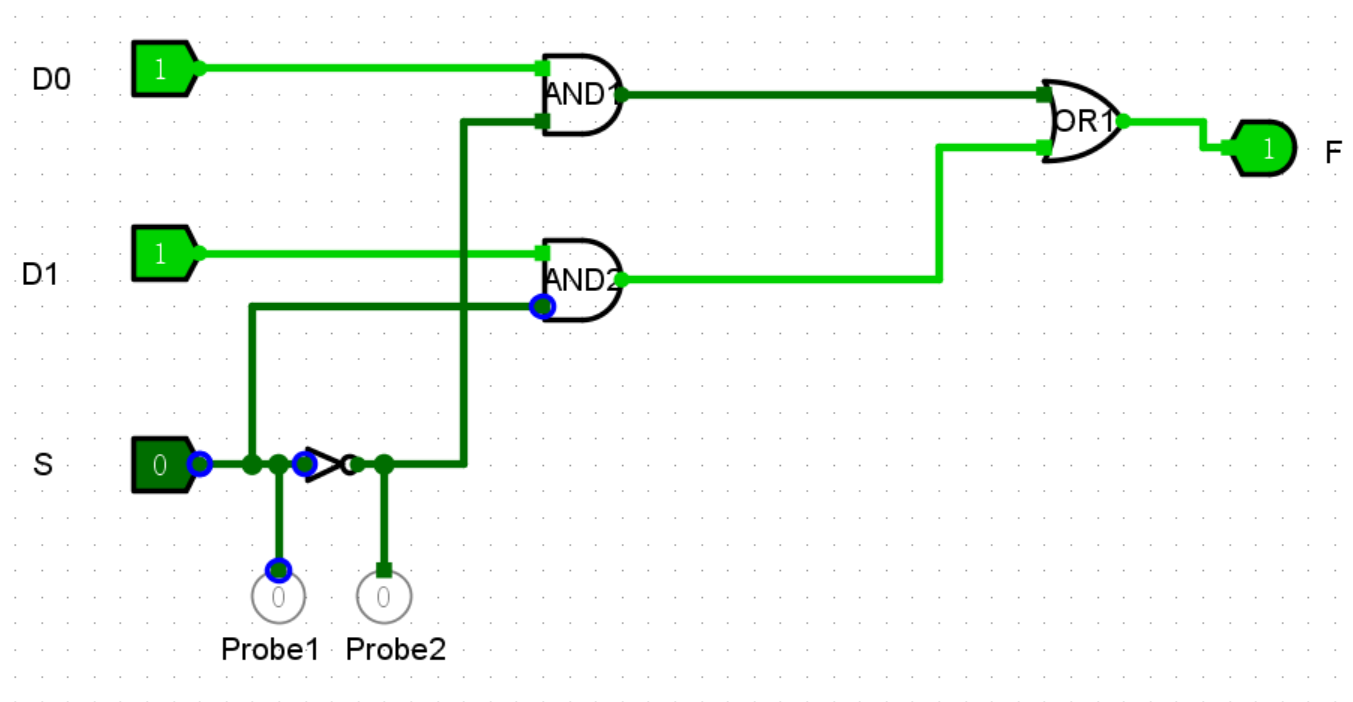
\includegraphics[width=0.4\textwidth]{3.6.3.png}
        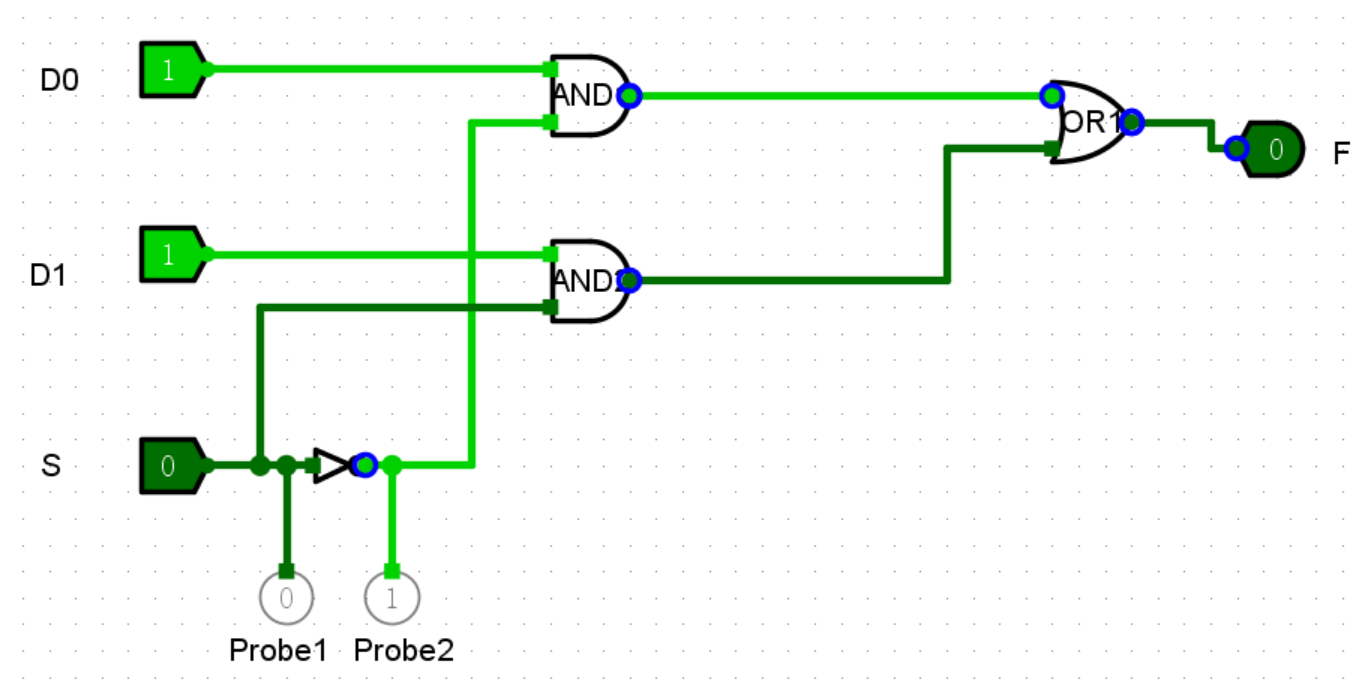
\includegraphics[width=0.4\textwidth]{3.6.4.png}
        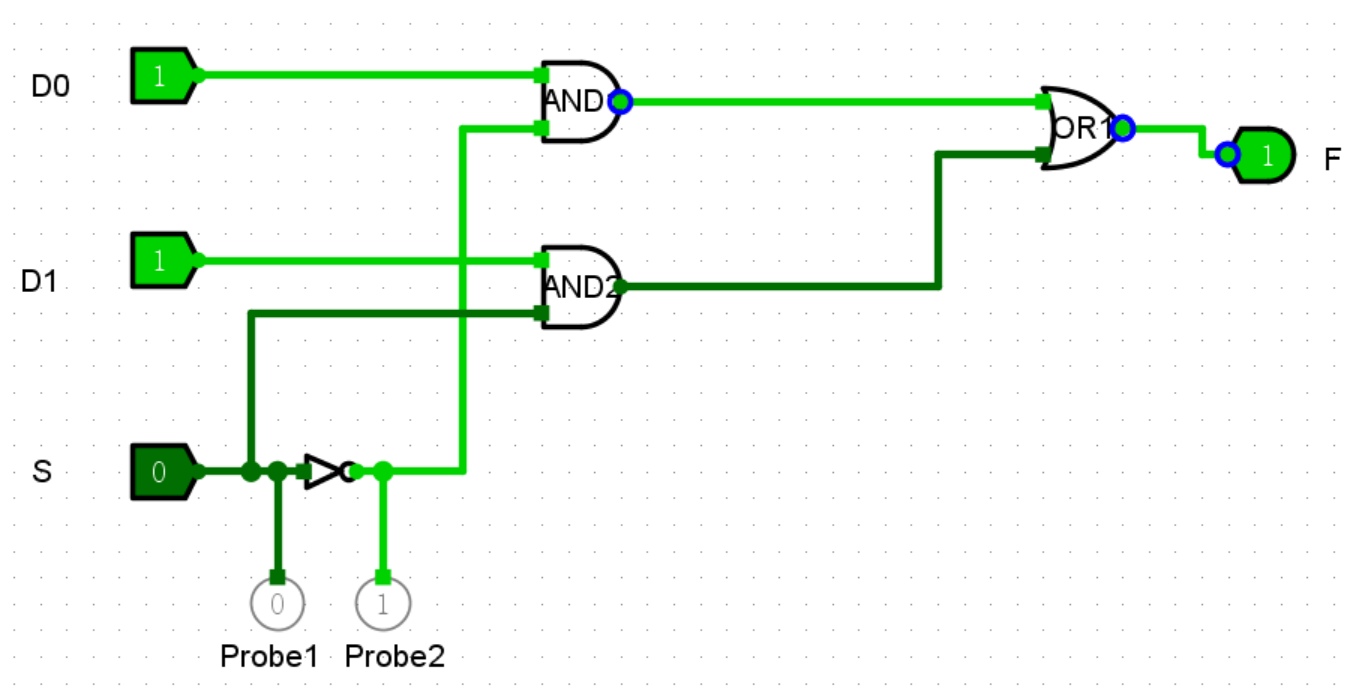
\includegraphics[width=0.4\textwidth]{3.6.5.png}
    \caption{2路选择器静态冒险检测图}
    \end{figure}
    \subsubsection{错误现象及分析}
    在完成实验的过程中,没有遇到任何错误。


    \subsection{利用传输门实现2路选择器}

    \subsubsection{整体方案设计}
    同实验3.
    
    \subsubsection{顶层模块设计}
    实验电路较为简单,不需要顶层模块设计图。

    \subsubsection{输入输出引脚}
    \begin{table}[H]
    \centering
    \begin{tabular}{|c|c|}
        \hline
        D0 D1 & 输入引脚 \\ \hline
        S & 使能端 \\ \hline 
        F   & 输出引脚 \\ \hline
    \end{tabular}
    \caption{2路选择器引脚作用}
    \end{table}

    \subsubsection{原理图和电路图}
    \begin{figure}[H]
    \centering
    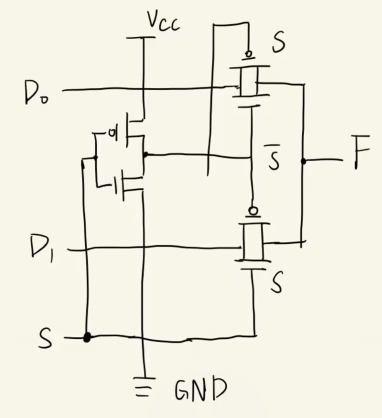
\includegraphics[width=0.8\textwidth]{4.4.1.png}
    \caption{2路选择器原理图}
    \end{figure}

    \begin{figure}[H]
    \centering
    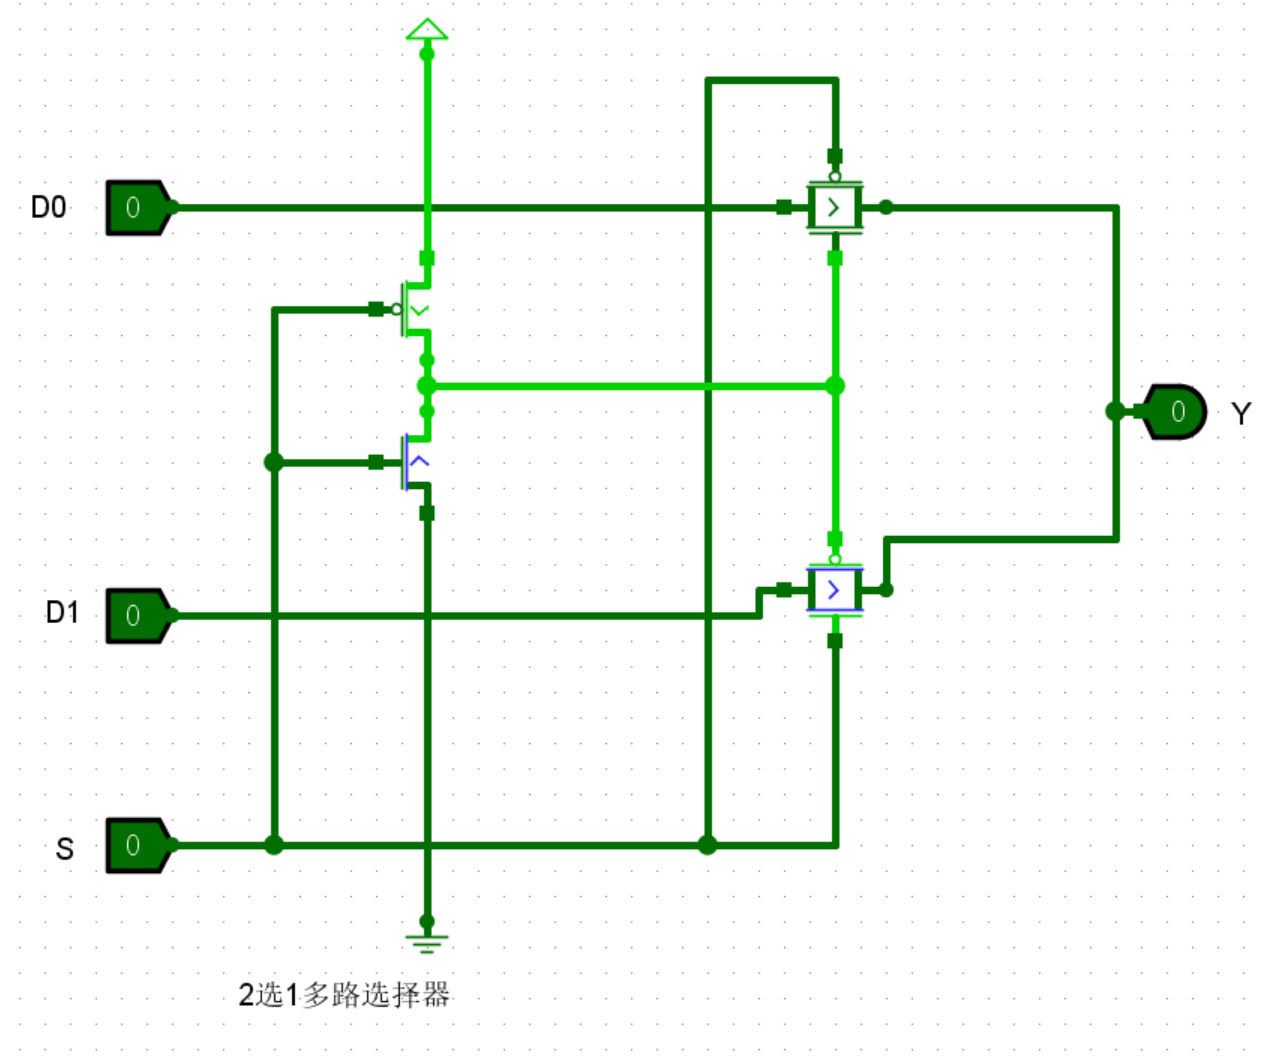
\includegraphics[width=0.8\textwidth]{4.4.2.png}
    \caption{2路选择器电路图}
    \end{figure}

    \subsubsection{仿真测试图}
    \begin{figure}[H]
    \centering
    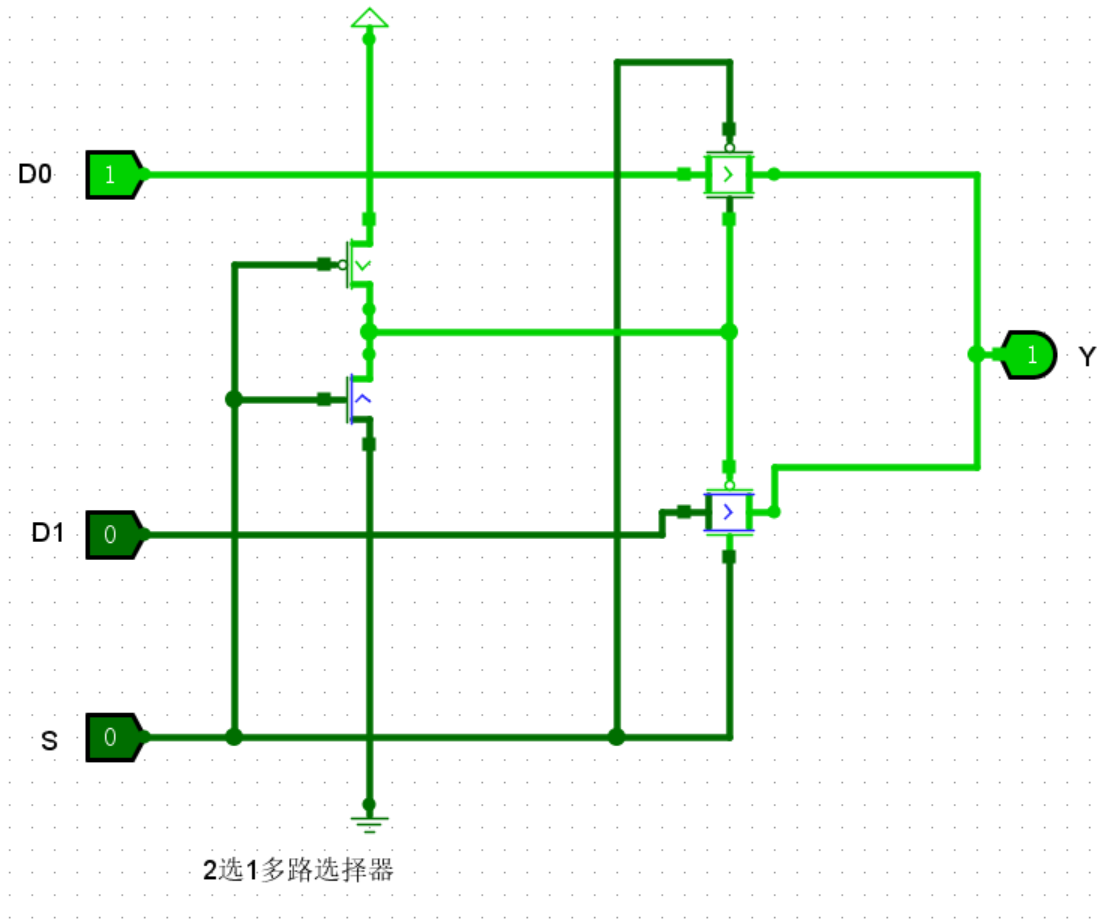
\includegraphics[width=0.4\textwidth]{4.5.1.png}
    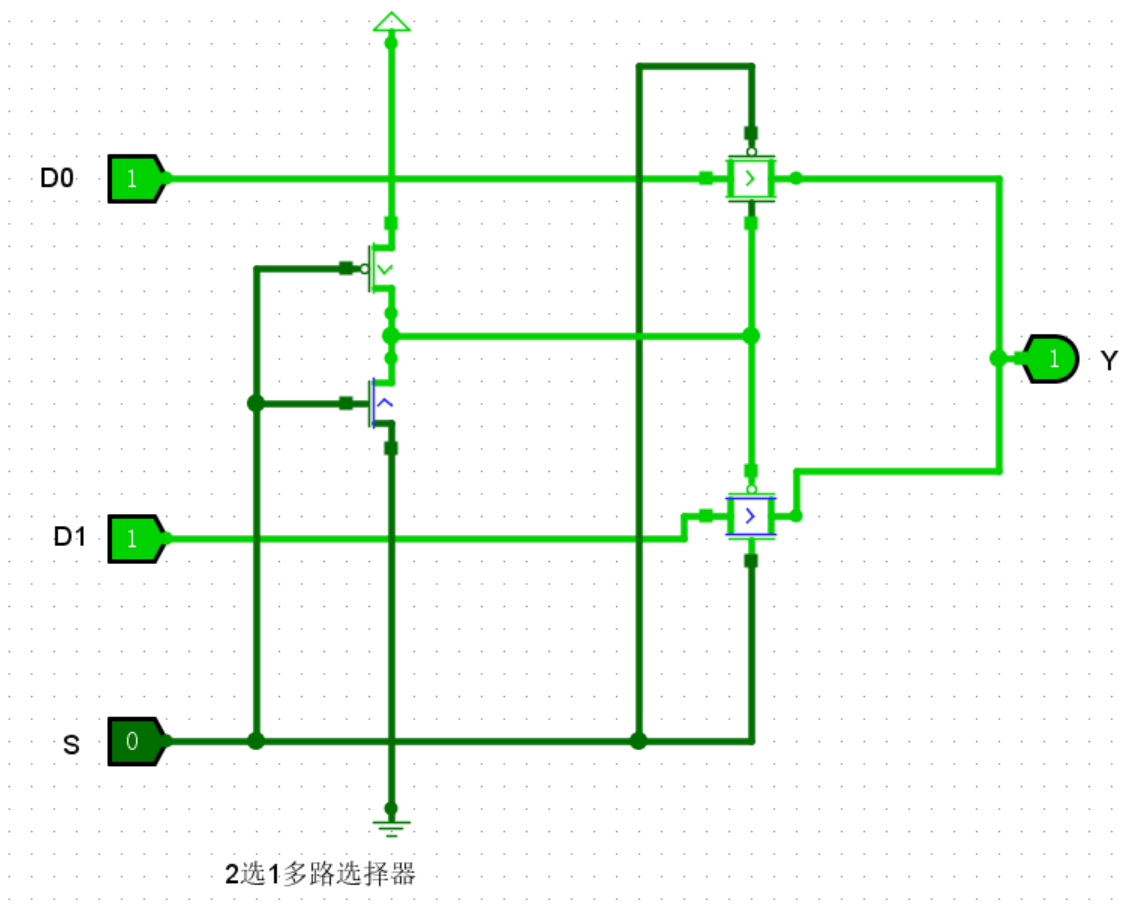
\includegraphics[width=0.4\textwidth]{4.5.2.png}
    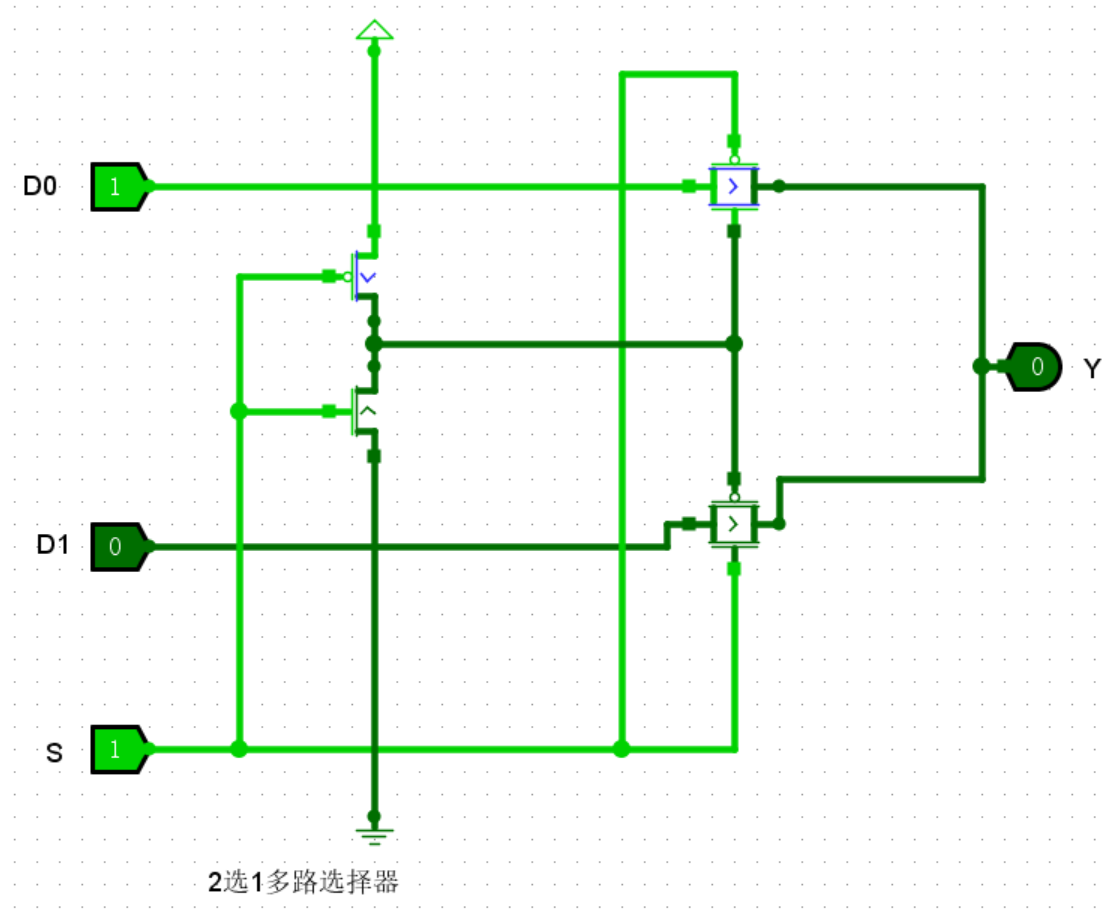
\includegraphics[width=0.4\textwidth]{4.5.3.png}
    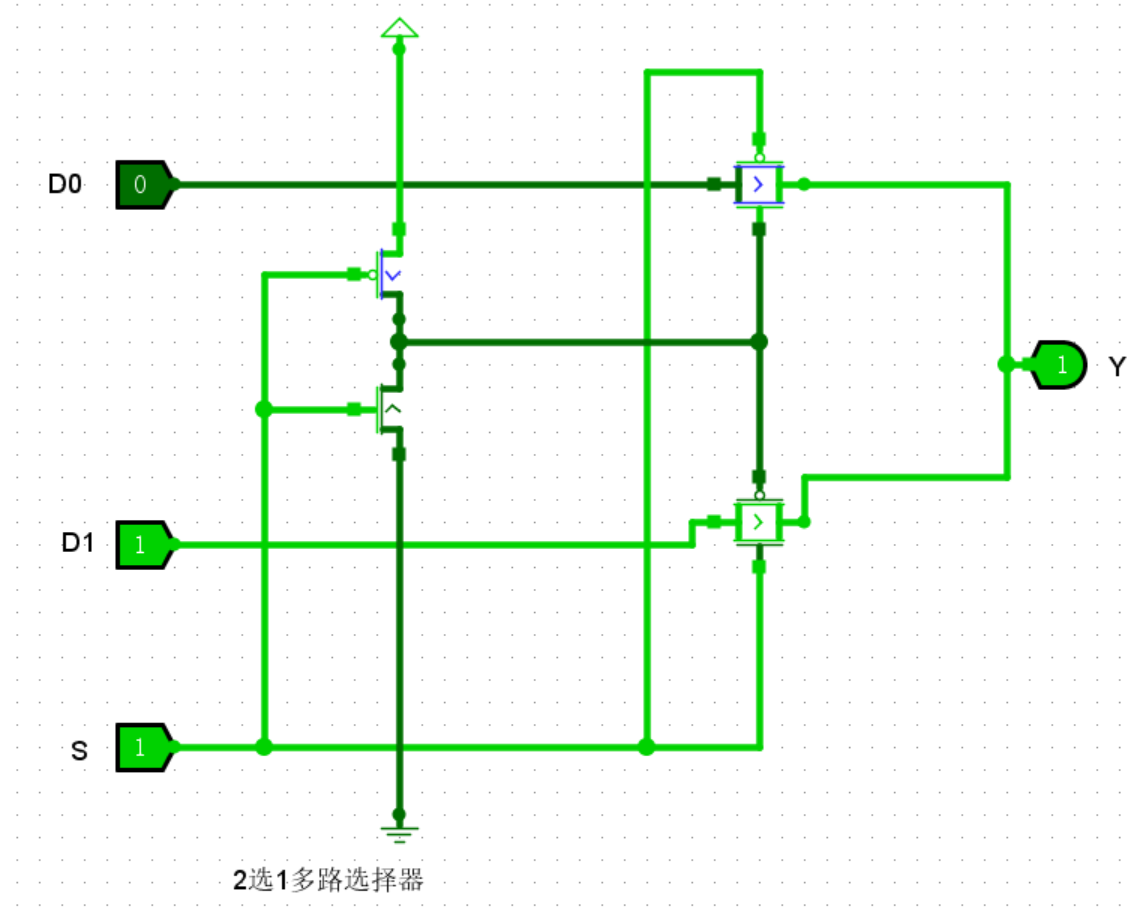
\includegraphics[width=0.4\textwidth]{4.5.4.png}
    \caption{2路选择器仿真测试图}
    \end{figure}

    \begin{table}[H]
    \centering
    \begin{tabular}{|c c c|c|}
        \hline
        D0 & D1 & S & F \\ \hline
        0 & 0 & 0 & 0 \\ \hline
        0 & 0 & 1 & 0 \\ \hline
        0 & 1 & 0 & 0 \\ \hline
        0 & 1 & 1 & 1 \\ \hline
        1 & 0 & 0 & 1 \\ \hline
        1 & 0 & 1 & 0 \\ \hline
        1 & 1 & 0 & 1 \\ \hline
        1 & 1 & 1 & 1 \\ \hline
    \end{tabular}
    \caption{2路选择器真值表}
    \end{table}

    \subsubsection{错误现象及分析}
    在完成实验的过程中,没有遇到任何错误。

    \subsection{使用组合电路分析功能设计2选1多路选择器}

    \subsubsection{操作方法}
    进入 Project - Analyze Circuit, 可以看到电路中已经定义的输入引脚和输出引脚,并且
    可以通过 Table, Expression, Minimized 三种方式自动生成电路。
    \begin{itemize}
        \item 方法一: 选择 Table, 可以看到当前电路的真值表,可以改变对应输出引脚的值,然后点击 Build
    Circuit 即可生成电路,如图 17 所示。 
        \item 方法二: 选择 Expression, 可以看到当前电路的逻辑表达式,可以改变逻辑表达式,然后点击 Build
    Circuit 即可生成电路,如图 18 所示。
        \item 方法三: 选择 Minimized, 可以看到当前电路的最小项和卡诺图,可以改变卡诺图中的若干项,然
    后点击 Build Circuit 即可生成电路,如图 19 所示。
    \end{itemize}
    
    \begin{figure}[H]
    \centering
    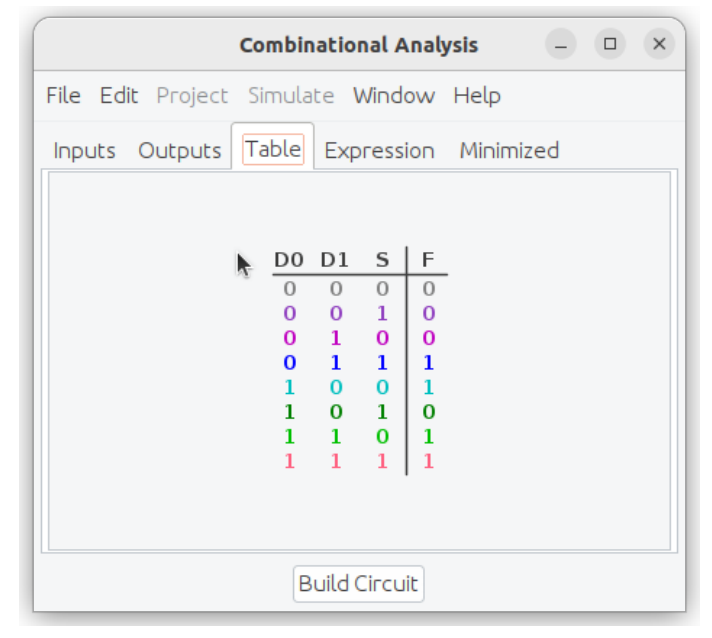
\includegraphics[width=0.8\textwidth]{5.1.1.png}
    \caption{ 2路选择器Table方法生成}
    \end{figure}

    \begin{figure}[H]
    \centering
    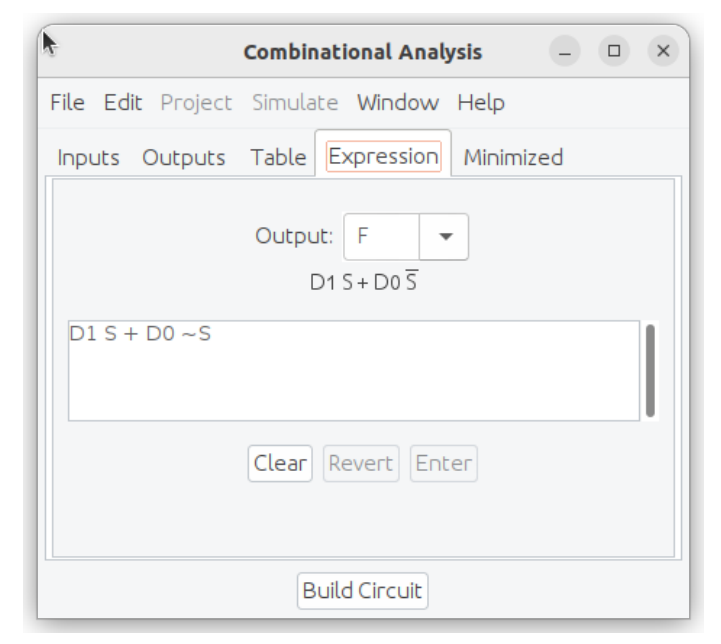
\includegraphics[width=0.8\textwidth]{5.1.2.png}
    \caption{ 2路选择器Expression方法生成}
    \end{figure}

    \begin{figure}[H]
    \centering
    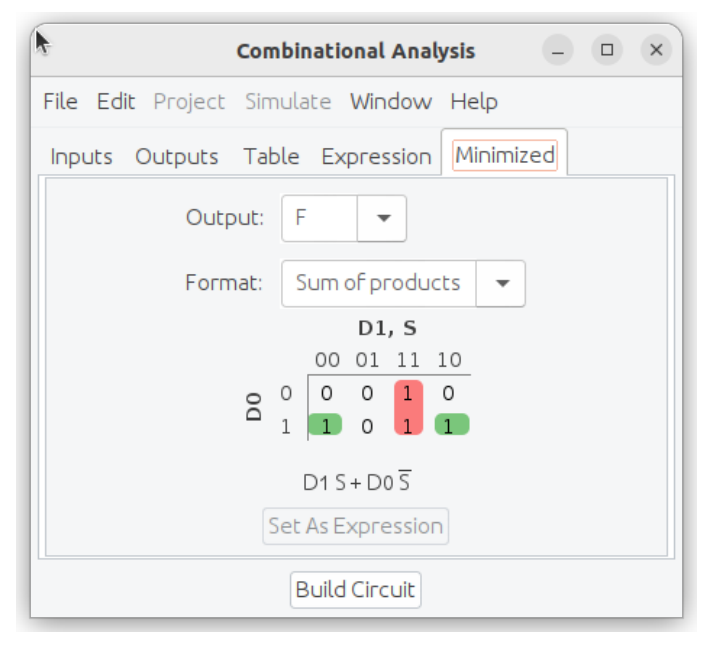
\includegraphics[width=0.8\textwidth]{5.1.3.png}
    \caption{ 2路选择器Minimized方法生成}
    \end{figure}

    \subsubsection{电路图}
    在生成电路图时,可以选择不同的电路图生成选项, 如图 20,图21,图22,图23 所示。
    \begin{figure}[H]
    \centering
    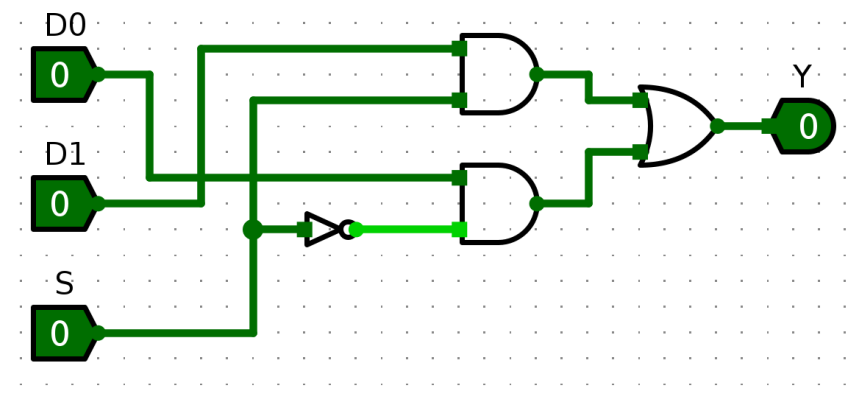
\includegraphics[width=0.8\textwidth]{5.2.1.png}   
    \caption{选择只使用2输入端逻辑门}
    \end{figure}

    \begin{figure}[H]
    \centering
    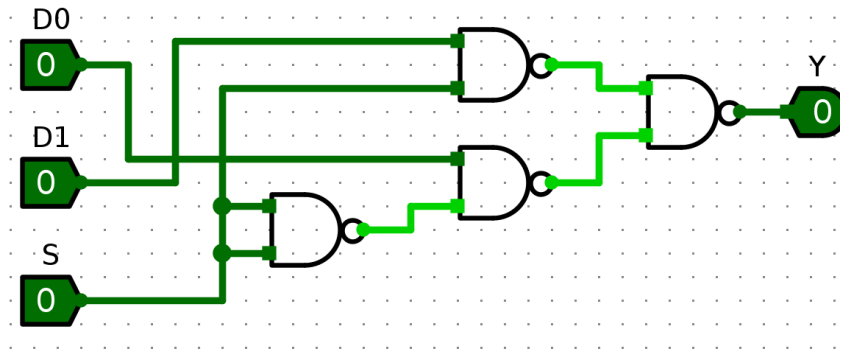
\includegraphics[width=0.8\textwidth]{5.2.2.png}
    \caption{选择只使用与非门}
    \end{figure}

    \begin{figure}[H]
    \centering
    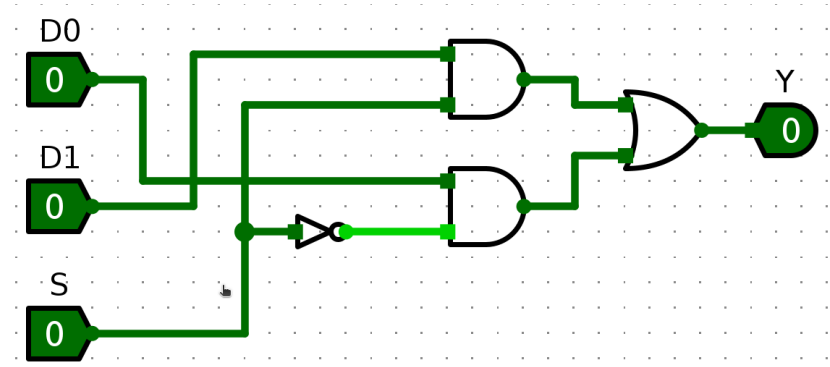
\includegraphics[width=0.8\textwidth]{5.2.3.png}
    \caption{选择两者都不使用}
    \end{figure}

    \begin{figure}[H]
    \centering
    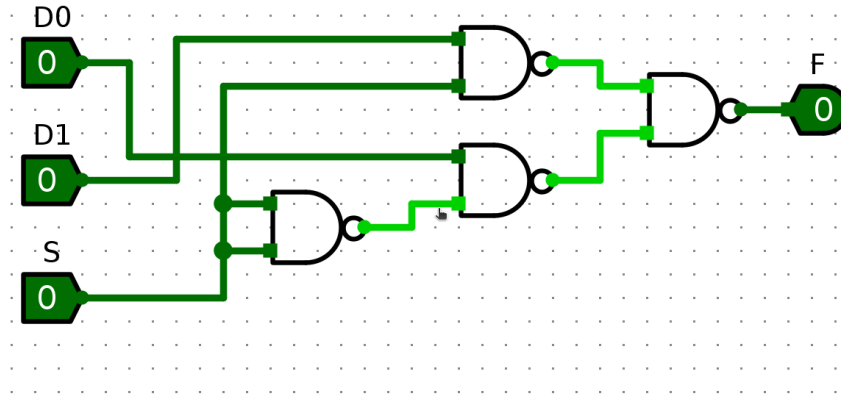
\includegraphics[width=0.8\textwidth]{5.2.4.png}
    \caption{同时使用2输入端逻辑门和与非门}
    \end{figure}

    \subsubsection{错误现象及分析}
    在完成实验的过程中,没有遇到任何错误。

    \subsection{使用2路选择器级联构建一个4路选择器}

    \subsubsection{整体方案设计}
    \begin{figure}[H]
    \centering
    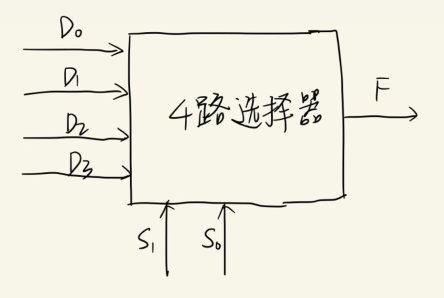
\includegraphics[width=0.8\textwidth]{6.1.png}
    \caption{4路选择器整体方案设计}
    \end{figure}
    
    \subsubsection{顶层模块设计}
    实验电路较为简单,不需要顶层模块设计图。

    \subsubsection{输入输出引脚}
    \begin{table}[H]
    \centering
    \begin{tabular}{|c|c|}
        \hline
        D0 D1 D2 D3 & 输入引脚 \\ \hline
        S0 S1 & 使能端 \\ \hline 
        F   & 输出引脚 \\ \hline
    \end{tabular}
    \caption{4路选择器引脚作用}
    \end{table}

    \subsubsection{原理图和电路图}
    \begin{figure}[H]
    \centering
    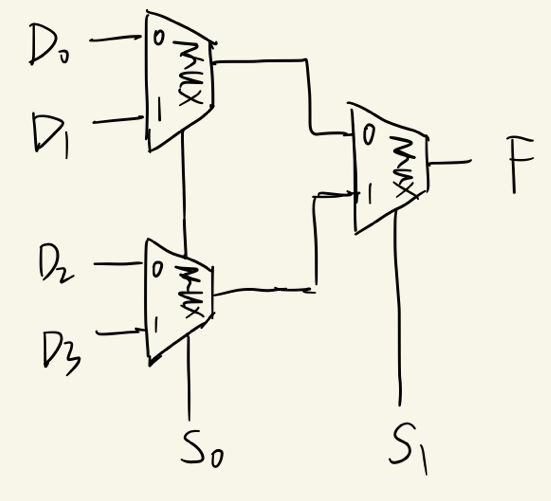
\includegraphics[width=0.8\textwidth]{6.4.1.png}
    \caption{4路选择器原理图}
    \end{figure}

    在该电路图中,用到的是\textbf{2路选择器(传输门实现)},外观如图26所示。

    \begin{figure}[H]
    \centering
    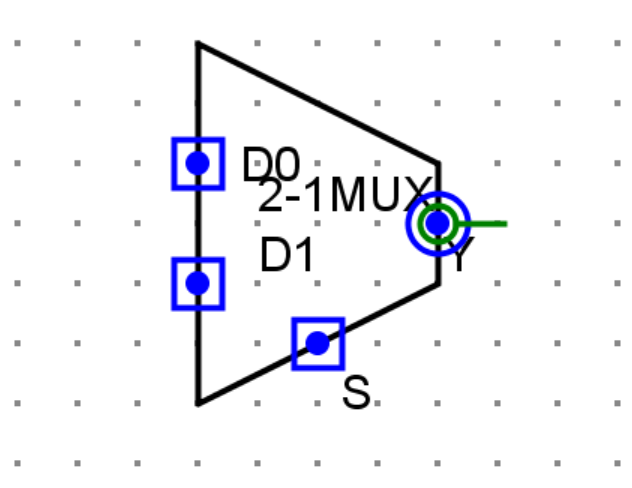
\includegraphics[width=0.8\textwidth]{6.4.2.png}
    \caption{2路选择器外观}
    \end{figure}


    \begin{figure}[H]
    \centering
    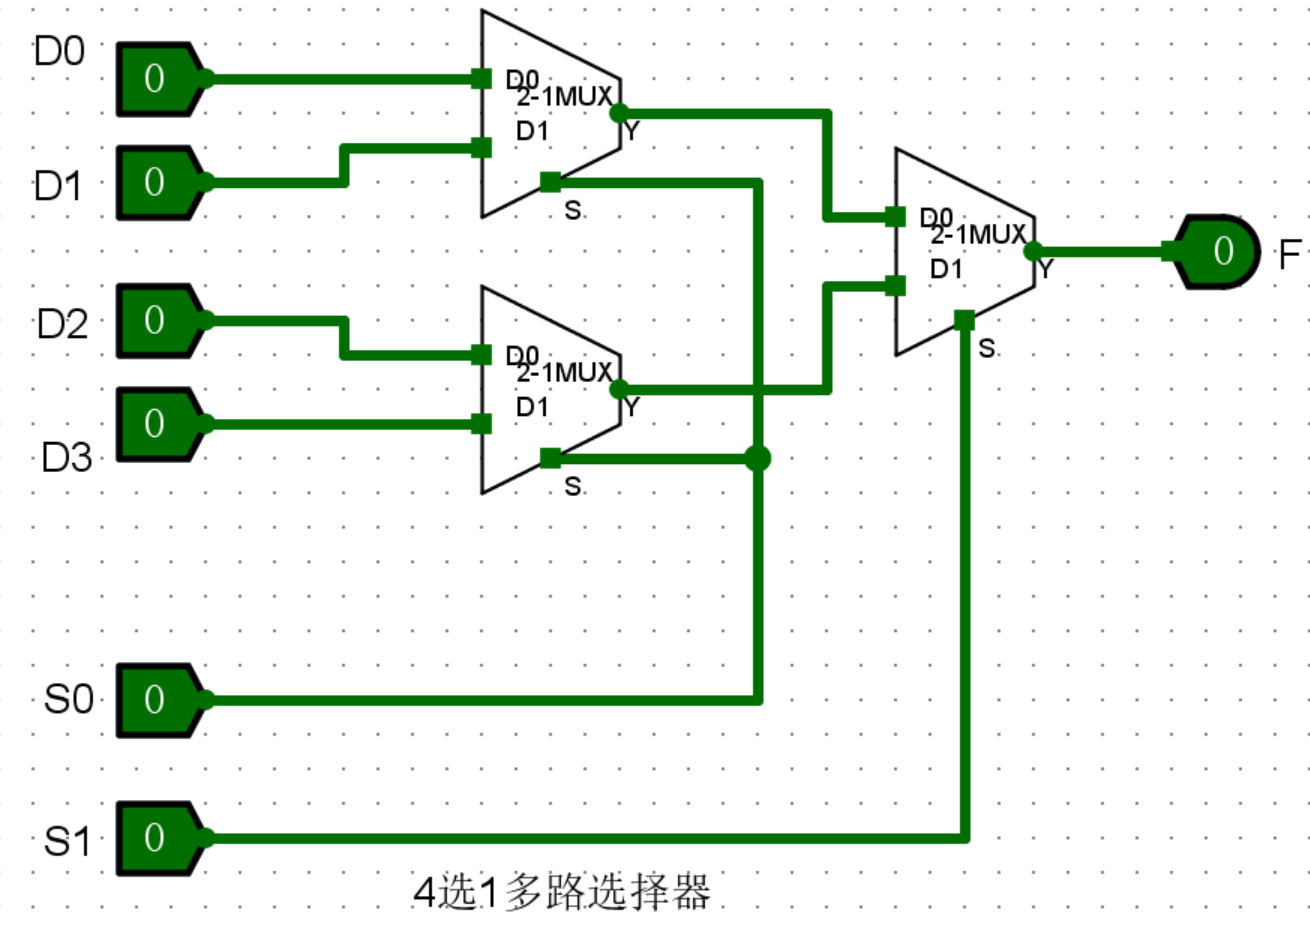
\includegraphics[width=0.8\textwidth]{6.4.3.png}
    \caption{4路选择器电路图}
    \end{figure}

    \subsubsection{仿真测试图}
    \begin{figure}[H]
    \centering
    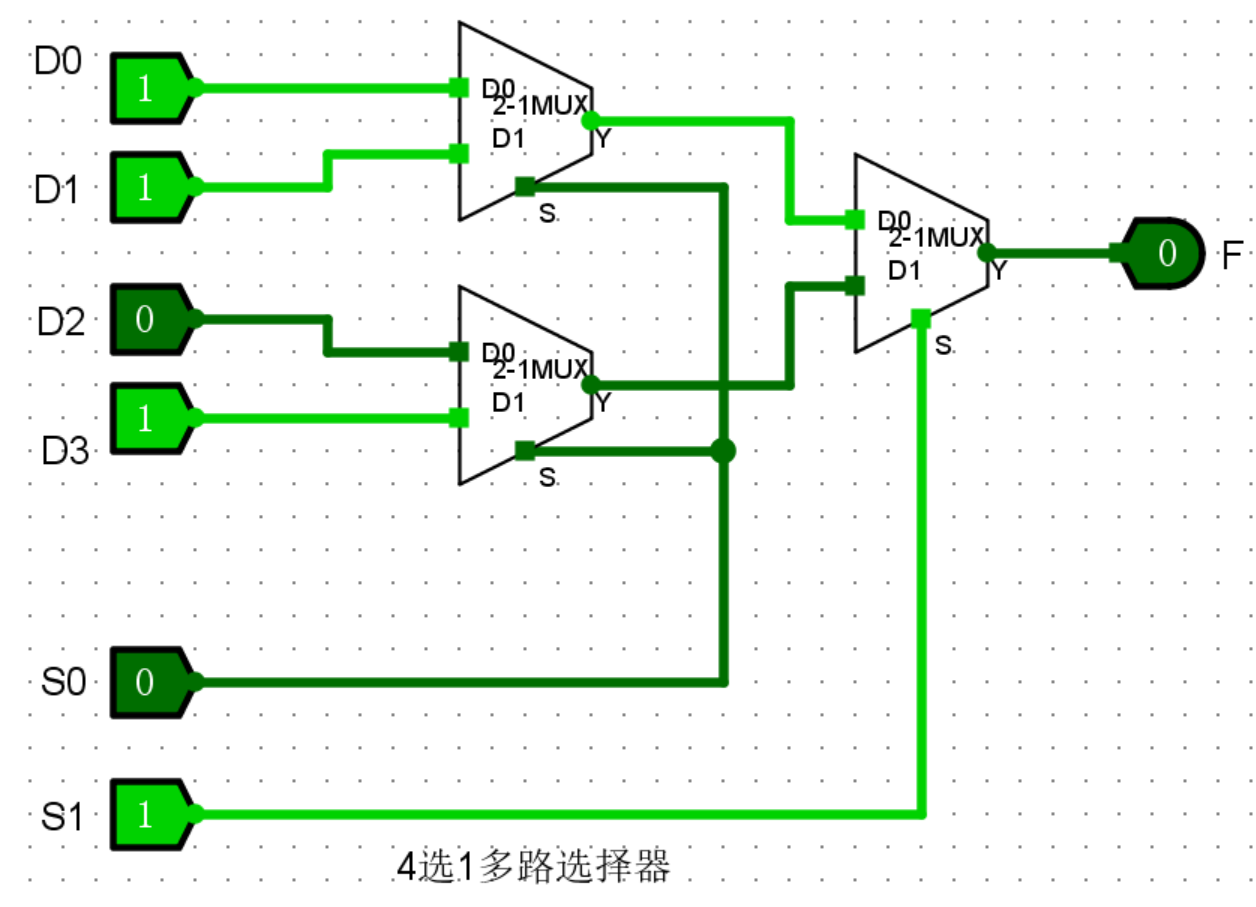
\includegraphics[width=0.4\textwidth]{6.5.1.png}
    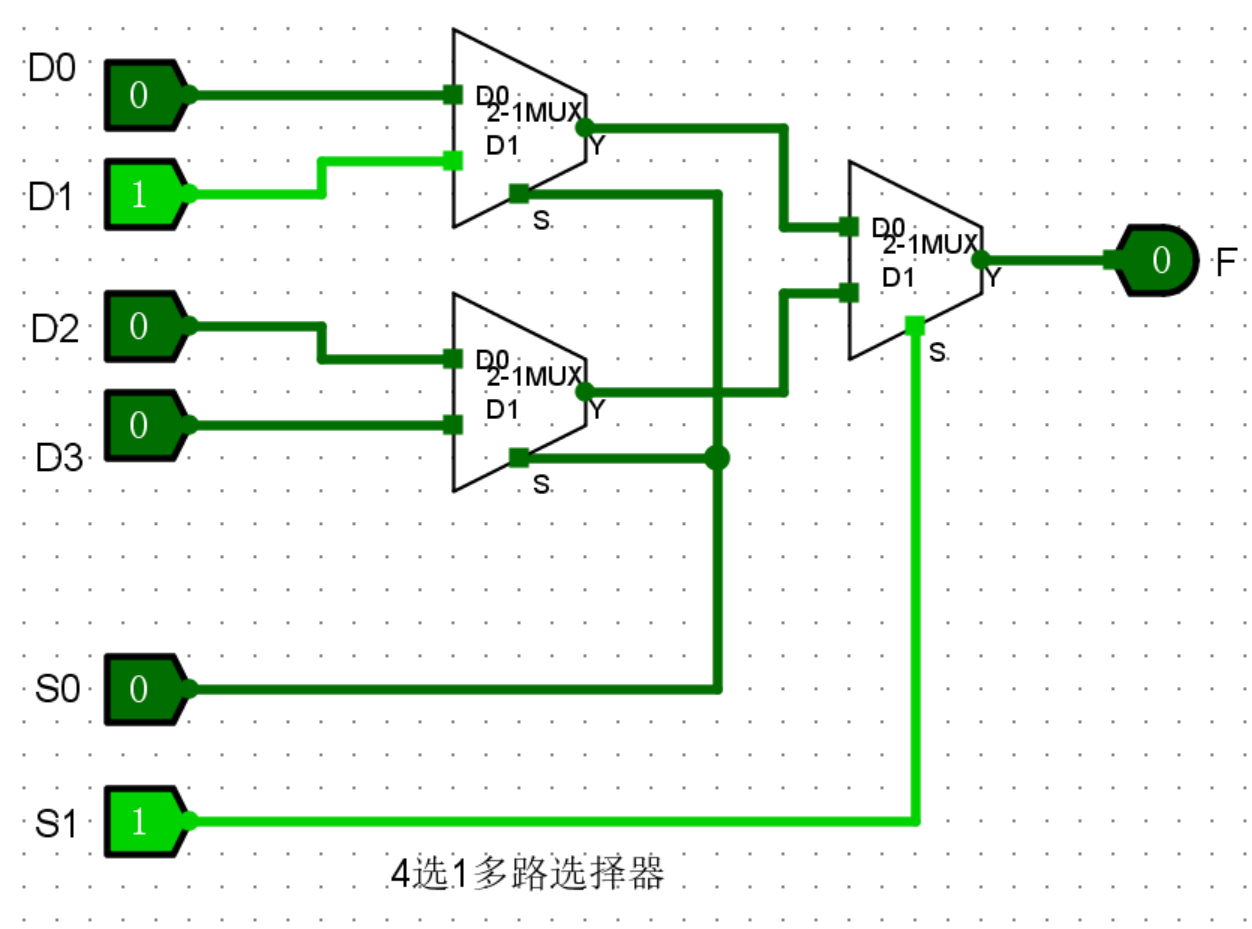
\includegraphics[width=0.4\textwidth]{6.5.2.png}
    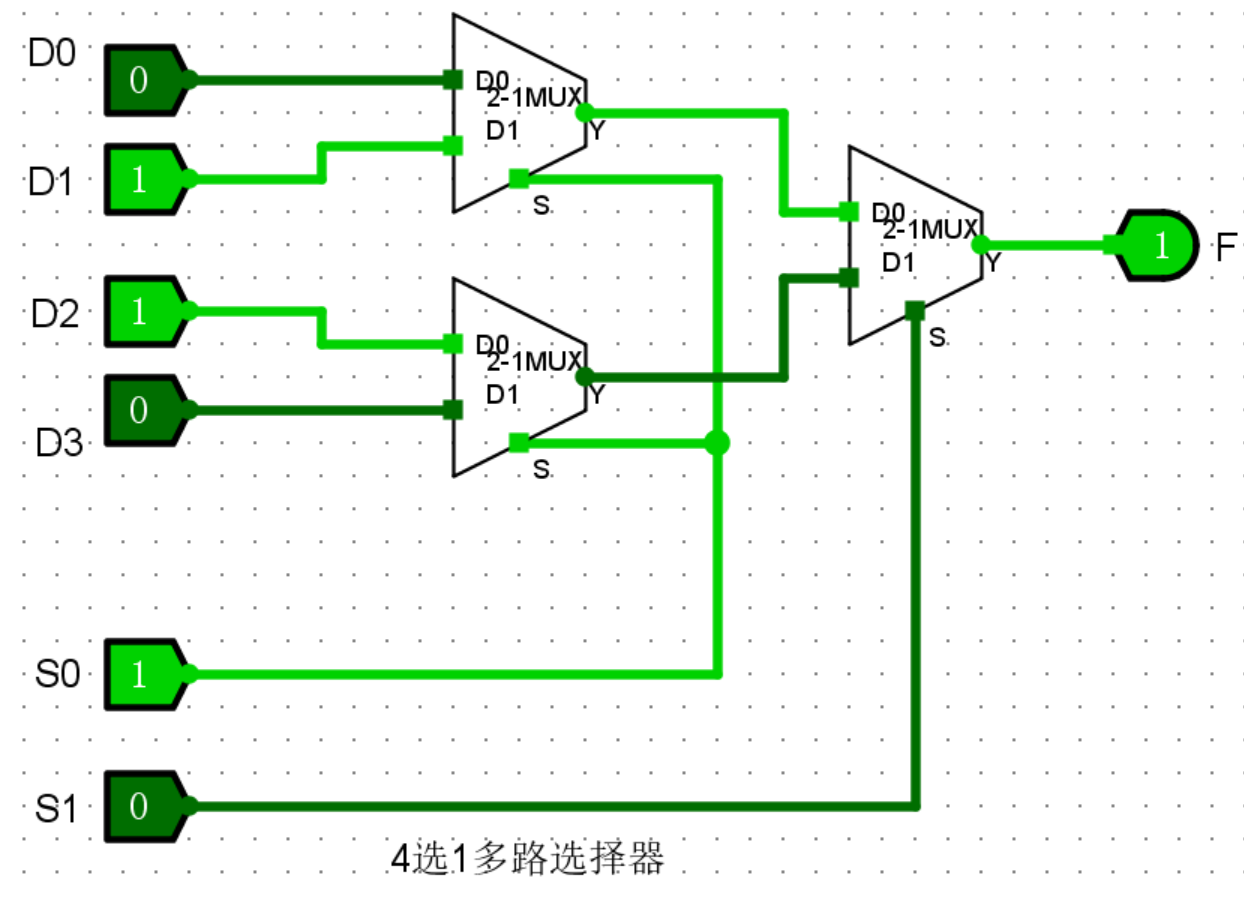
\includegraphics[width=0.4\textwidth]{6.5.3.png}
    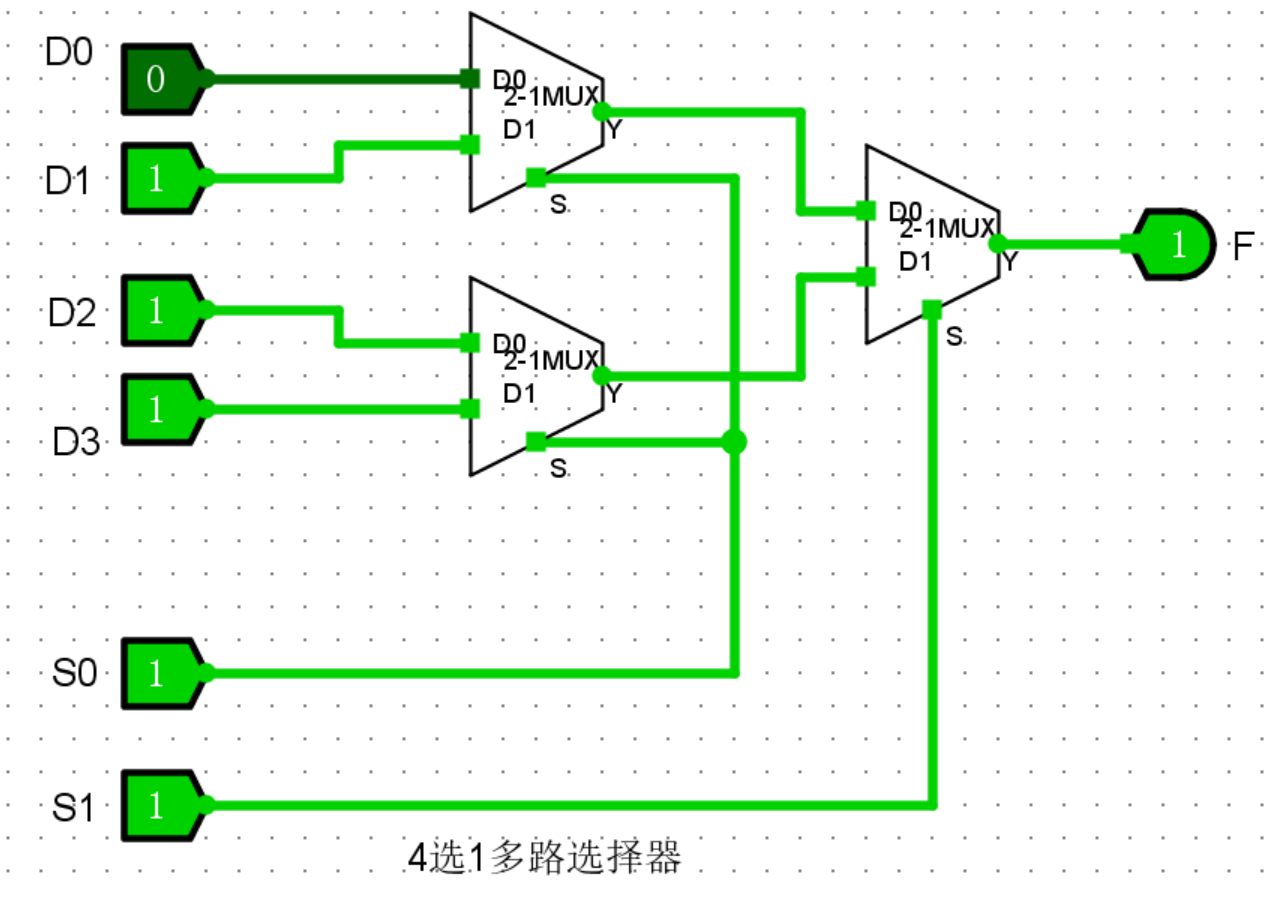
\includegraphics[width=0.4\textwidth]{6.5.4.png}
    \caption{4路选择器仿真测试图}
    \end{figure}

    \begin{table}[H]
    \centering
    \begin{tabular}{|c c c c|c c|c|}
        \hline
        D0 & D1 & D2 & D3 & S0 & S1 & F \\ \hline
        0 & x & x & x & 0 & 0 & 0 \\ \hline
        1 & x & x & x & 0 & 0 & 1 \\ \hline
        x & 0 & x & x & 1 & 0 & 0 \\ \hline
        x & 1 & x & x & 1 & 0 & 1 \\ \hline
        x & x & 0 & x & 0 & 1 & 0 \\ \hline
        x & x & 1 & x & 0 & 1 & 1 \\ \hline
        x & x & x & 0 & 1 & 1 & 0 \\ \hline
        x & x & x & 1 & 1 & 1 & 1 \\ \hline
    \end{tabular}
    \caption{4路选择器真值表}
    \end{table}

    \subsubsection{错误现象及分析}
    在完成实验的过程中,没有遇到任何错误。


    \subsection{隧道和集线器部件实验}

    \subsubsection{整体方案设计}
    \begin{figure}[H]
    \centering
    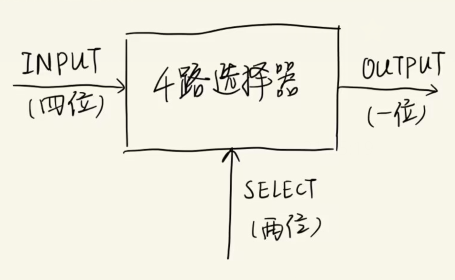
\includegraphics[width=0.8\textwidth]{7.1.png}
    \caption{4路选择器整体方案设计}
    \end{figure}
    
    \subsubsection{顶层模块设计}
    实验电路较为简单,不需要顶层模块设计图。

    \subsubsection{输入输出引脚}
    \begin{table}[H]
    \centering
    \begin{tabular}{|c|c|}
        \hline
        INPUT & 输入引脚 \\ \hline
        SELECT & 使能端 \\ \hline 
        OUTPUT & 输出引脚 \\ \hline
    \end{tabular}
    \caption{4路选择器引脚作用}
    \end{table}

    \subsubsection{原理图和电路图}
    原理图除集成引脚外,和图 25 相同。

    \begin{figure}[H]
    \centering
    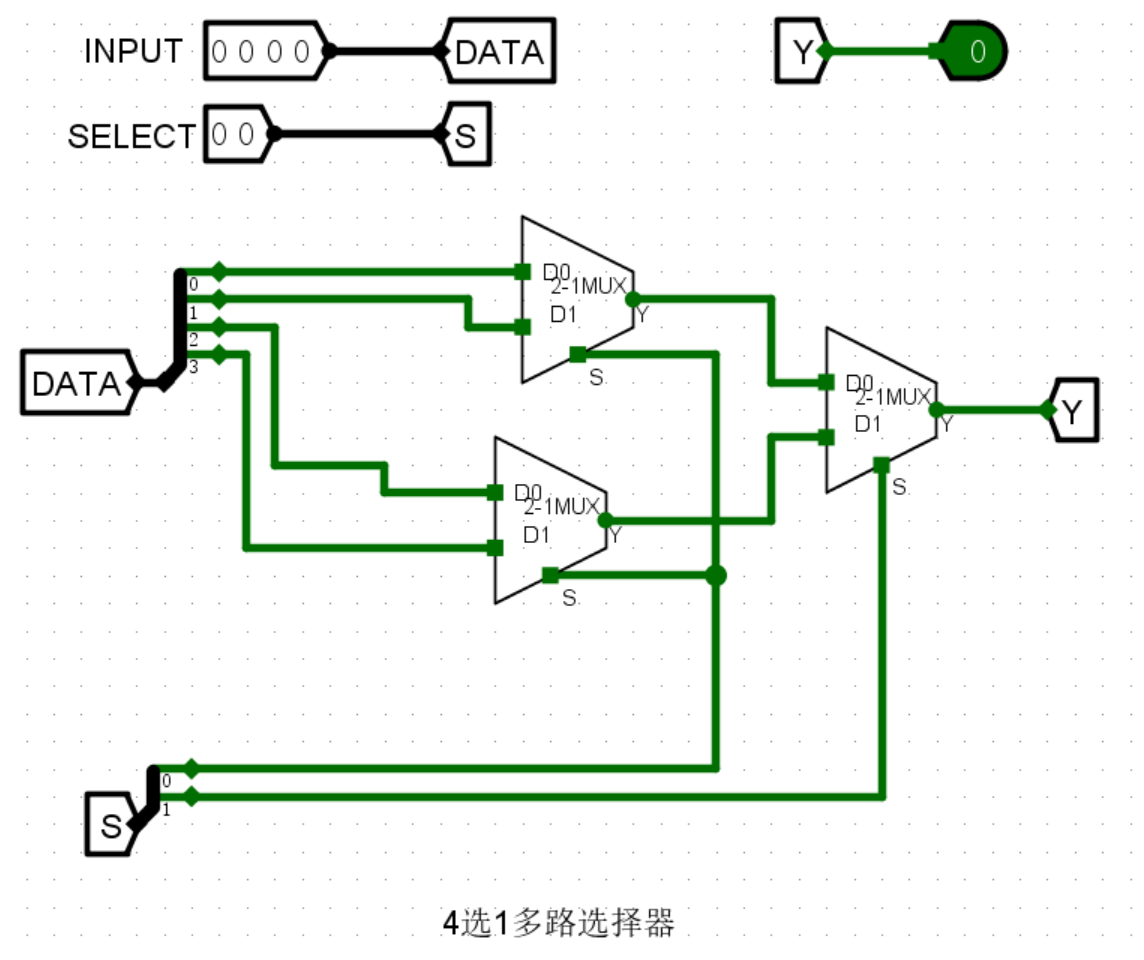
\includegraphics[width=0.8\textwidth]{7.4.1.png}
    \caption{4路选择器电路图}
    \end{figure}

    \subsubsection{仿真测试图}
    \begin{figure}[H]
    \centering
    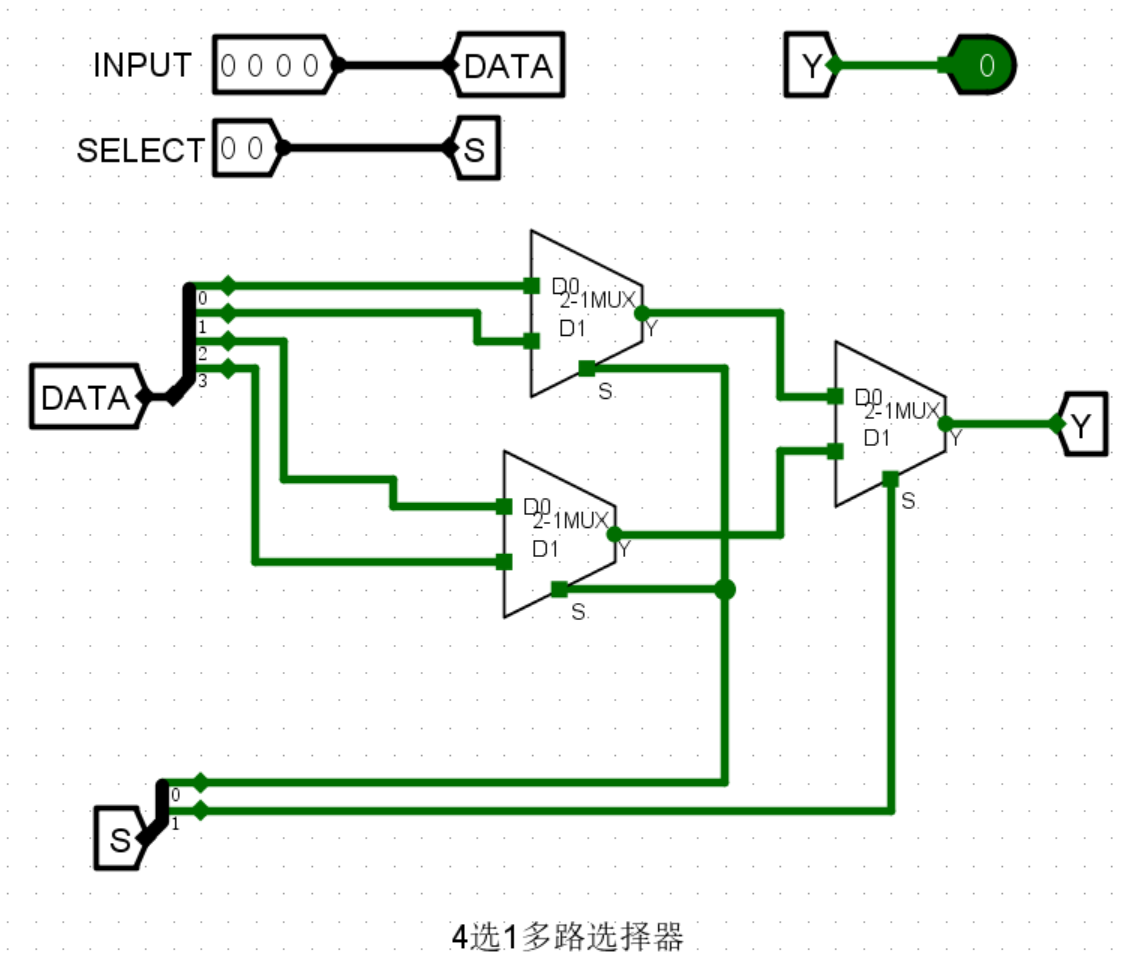
\includegraphics[width=0.4\textwidth]{7.5.1.png}
    \includegraphics[width=0.4\textwidth]{7.5.2.png}
    \includegraphics[width=0.4\textwidth]{7.5.3.png}
    \includegraphics[width=0.4\textwidth]{7.5.4.png}
    \caption{4路选择器仿真测试图}
    \end{figure}

    \begin{table}[H]
    \centering
    \begin{tabular}{|c c c c|c c|c|}
        \hline
        D0 & D1 & D2 & D3 & S0 & S1 & F \\ \hline
        0 & x & x & x & 0 & 0 & 0 \\ \hline
        1 & x & x & x & 0 & 0 & 1 \\ \hline
        x & 0 & x & x & 1 & 0 & 0 \\ \hline
        x & 1 & x & x & 1 & 0 & 1 \\ \hline
        x & x & 0 & x & 0 & 1 & 0 \\ \hline
        x & x & 1 & x & 0 & 1 & 1 \\ \hline
        x & x & x & 0 & 1 & 1 & 0 \\ \hline
        x & x & x & 1 & 1 & 1 & 1 \\ \hline
    \end{tabular}
    \caption{4路选择器真值表}
    \end{table}

    \subsubsection{错误现象及分析}
    在完成实验的过程中,没有遇到任何错误。


    \section{思考题}

    \subsection{将实验中设计的或门作为子电路应用到2-1MUX-hazard电路中}
    修改后的电路图如图 32 所示。
    \begin{figure}[H]
    \centering
    \includegraphics[width=0.8\textwidth]{8.1.png}
    \caption{修改后的2-1MUX-hazard电路图}
    \end{figure}


    \subsection{修改现有电路设计实现4位4选1多路选择器}

    将实验7-隧道和集线器部件实验中最终呈现的电路图中的输入引脚 INPUT 的位宽设置
    为 16,选择引脚 SELECT 不变,输出引脚 OUTPUT 的位宽设置为 4,并相应地修改电路
    中选择器的位宽,即可实现 4 位 4 选 1 多路选择器,如图33所示。
    \begin{figure}[H]
    \centering
    \includegraphics[width=0.8\textwidth]{9.1.png}
    \caption{4 位 4 选 1 多路选择器电路图}
    \end{figure}
    其中MUX为Logisim中的位宽为4的2选1多路选择器。
    图34为该电路的仿真测试图。

    \begin{figure}[H]
    \centering
    \includegraphics[width=0.4\textwidth]{9.2.1.png}
    \includegraphics[width=0.4\textwidth]{9.2.2.png}
    \includegraphics[width=0.4\textwidth]{9.2.3.png}
    \includegraphics[width=0.4\textwidth]{9.2.4.png}
    \caption{4位4选1多路选择器仿真测试图}
    \end{figure}

    \subsection{设计并实现4位二进制数的奇偶校验位生成电路}
    \subsubsection{整体方案设计}
    \begin{figure}[H]
    \centering
    \includegraphics[width=0.8\textwidth]{10.1.png}
    \caption{4位二进制数的奇偶校验位生成电路整体方案设计图}
    \end{figure}
    \subsubsection{输入输出引脚}
    \begin{table}[H]
        \centering
        \begin{tabular}{|c|c|}
            \hline
            INPUT & 输入引脚(4位二进制数) \\ \hline
            ODD & 奇校验位输出引脚 \\ \hline 
            OUTPUT & 偶校验位输出引脚 \\ \hline
        \end{tabular}
        \caption{4位二进制数的奇偶校验位生成电路引脚作用}
        \end{table}
    \subsubsection{原理图和电路图}

    \begin{figure}[H]
    \centering
    \includegraphics[width=0.8\textwidth]{10.3.1.png}
    \caption{4位二进制数的奇偶校验位生成电路原理图}
    \end{figure}

    \begin{figure}[H]
        \centering
        \includegraphics[width=0.8\textwidth]{10.3.2.png}
        \caption{4位二进制数的奇偶校验位生成电路电路图}
        \end{figure}
    \subsubsection{仿真测试图}

    \begin{figure}[H]
        \centering
        \includegraphics[width=0.4\textwidth]{10.4.1.png}
        \includegraphics[width=0.4\textwidth]{10.4.2.png}
        \includegraphics[width=0.4\textwidth]{10.4.3.png}
        \includegraphics[width=0.4\textwidth]{10.4.4.png}
        \caption{4位二进制数的奇偶校验位生成电路电路图仿真测试图}
        \end{figure}

    \begin{table}[H]
    \centering
    \begin{tabular}{|c c c c|c c|}
        \hline
        A & B & C & D & EVEN & ODD  \\ \hline
        0 & 0 & 0 & 0 & 0 & 1  \\ \hline
        0 & 0 & 0 & 1 & 1 & 0  \\ \hline
        0 & 0 & 1 & 0 & 1 & 0  \\ \hline
        0 & 0 & 1 & 1 & 0 & 1  \\ \hline
        0 & 1 & 0 & 0 & 1 & 0  \\ \hline
        0 & 1 & 0 & 1 & 0 & 1  \\ \hline
        0 & 1 & 1 & 0 & 0 & 1  \\ \hline
        0 & 1 & 1 & 1 & 1 & 0  \\ \hline
        1 & 0 & 0 & 0 & 1 & 0  \\ \hline
        1 & 0 & 0 & 1 & 0 & 1  \\ \hline
        1 & 0 & 1 & 0 & 0 & 1  \\ \hline
        1 & 0 & 1 & 1 & 1 & 0  \\ \hline
        1 & 1 & 0 & 0 & 0 & 1  \\ \hline
        1 & 1 & 0 & 1 & 1 & 0  \\ \hline
        1 & 1 & 1 & 0 & 1 & 0  \\ \hline
        1 & 1 & 1 & 1 & 0 & 1  \\ \hline
    \end{tabular}
    \caption{4位二进制数的奇偶校验位生成电路真值表}
    \end{table}
    逻辑表达式为EVEN=$A\oplus B\oplus C\oplus D,$EVEN = $\overline{A\oplus B\oplus C\oplus D}  $。
\end{document}